% ----- auto-generated from week_07/Week*.html via pandoc -----
\chapter{Backstepping Control (Week 7)}
\labch{week_07}



Recursive Lyapunov Design for Nonlinear Systems

M.Sc. Control for Robots --- AY 2025--26\\
Duration: 3 Hours (Lecture + Hands-on Lab)

\section{Overview}

\subsection{Week 5 Recall: Robust Control --- Exam Practice (20 min)}

\subsection{Question 1 --- Robust Sliding-Mode Analysis}

Consider a manipulator with model uncertainty:

\[
                M(q)\ddot{q} + C(q,\dot{q})\dot{q} + G(q) = \tau + d(t), \qquad \|d(t)\| \le d_{\max}
            \]

The robust controller is:

\[
                \tau = \hat{M}(q)\bigl[\ddot{q}_d + K_D \dot{e} + K_P e\bigr] + \hat{C}\dot{q} + \hat{G} + \tau_{\text{robust}}
            \]

with the robust term

\[
                \tau_{\text{robust}} = \rho(t)\,\frac{s}{\|s\|}, \qquad s = \dot{e} + \Lambda\, e
            \]

where \(e = q_d - q\), \(\dot{e} = \dot{q}_d - \dot{q}\), and \(\Lambda \succ 0\).

\subsubsection{Model Answer --- Closed-Loop Error Dynamics}

\textbf{Step 1 --- Substitution.} Write the true dynamics as
\(M\ddot{q} = \tau + d - C\dot{q} - G\).
Substitute the controller:

\[
                    M\ddot{q} = \hat{M}(\ddot{q}_d + K_D\dot{e} + K_P e) + \hat{C}\dot{q} + \hat{G}
                    + \rho\frac{s}{\|s\|} + d - C\dot{q} - G
                \]

Define the model errors
\(\tilde{M} = M - \hat{M}\), \(\tilde{C} = C - \hat{C}\), \(\tilde{G} = G - \hat{G}\),
and let the lumped uncertainty be

\[
                    \eta(t) = \tilde{M}\ddot{q} + \tilde{C}\dot{q} + \tilde{G} - d(t)
                \]

\textbf{Step 2 --- Error dynamics.}
With \(\ddot{e} = \ddot{q}_d - \ddot{q}\) and after algebraic manipulation:

\[
                    M\ddot{e} + (C + M K_D)\dot{e} + M K_P e = -\eta(t) + \rho\frac{s}{\|s\|}
                \]

In terms of the composite variable \(s = \dot{e} + \Lambda e\):

\[
                    M\dot{s} = -Cs + \eta(t) + \rho\frac{s}{\|s\|}
                \]

(using the choice \(K_D = \Lambda\), \(K_P = \dot{\Lambda}\) to simplify).

\textbf{Step 3 --- Lyapunov analysis.} Choose
\(V = \tfrac{1}{2}\,s^T M\, s\). Then:

\[
                    \dot{V} = s^T M\dot{s} + \tfrac{1}{2}\,s^T\dot{M}\,s
                    = s^T\!\bigl[-Cs + \eta + \rho\tfrac{s}{\|s\|}\bigr] + \tfrac{1}{2}\,s^T\dot{M}\,s
                \]

Using the skew-symmetry property \(s^T(\dot{M} - 2C)s = 0\):

\[
                    \dot{V} = s^T\eta + \rho\|s\|
                \]

Since \(\tau_{\text{robust}}\) opposes the uncertainty
(note the sign convention: \(\rho \frac{s}{\|s\|}\) acts in the direction of \(s\), so the correct robust term to \emph{counteract} uncertainty is \(\tau_{\text{robust}} = -\rho \frac{s}{\|s\|}\)). Re-doing with the standard sign:

\[
                    \dot{V} = s^T\eta - \rho\|s\| \le \|\eta\|\,\|s\| - \rho\|s\| = (\|\eta\| - \rho)\|s\|
                \]

\textbf{Conclusion:} If \(\rho(t) \ge \|\eta(t)\|\), then \(\dot{V} \le 0\) and the tracking error \(s \to 0\). The sliding variable converges, guaranteeing bounded tracking despite uncertainty. By Barbalat\textquotesingle s lemma, \(s(t) \to 0\) asymptotically, which implies \(e(t) \to 0\) exponentially since \(\dot{e} = s - \Lambda e\) is a stable filter.

\subsection{Question 2 --- Robust vs. Adaptive: Mathematical Comparison}

\subsubsection{Model Answer}

\textbf{Adaptive control} uses an augmented Lyapunov function:

\[
                    V_{\text{adaptive}} = \frac{1}{2}\,s^T M\, s + \frac{1}{2}\,\tilde{\theta}^T \Gamma^{-1} \tilde{\theta}
                \]

where \(\tilde{\theta} = \theta - \hat{\theta}\) is the parameter estimation error
and \(\Gamma \succ 0\) is the adaptation gain matrix. The adaptation law
\(\dot{\hat{\theta}} = \Gamma\, Y^T s\) is designed so that
the cross-term \(s^T Y \tilde{\theta}\) in \(\dot{V}\) cancels exactly with
\(\tilde{\theta}^T \Gamma^{-1}\dot{\hat{\theta}}\), yielding:

\[
                    \dot{V}_{\text{adaptive}} = -s^T K_D\, s \le 0
                \]

\textbf{Robust control} uses a simpler Lyapunov function:

\[
                    V_{\text{robust}} = \frac{1}{2}\,s^T M\, s
                \]

No parameter estimation is required because the robust term directly dominates
the uncertainty via the bound \(\rho \ge \|\eta\|\):

\[
                    \dot{V}_{\text{robust}} \le -(\rho - \|\eta\|)\|s\| \le 0
                \]

\textbf{Why robust control does not need parameter estimation:}
Instead of identifying \emph{what} the uncertainty is (as adaptive control does), robust control only needs to know \emph{how large} the uncertainty can be. It overpowers the worst case with a dominating gain \(\rho\).

\textbf{Trade-off:}

\begin{table}[ht]\footnotesize\centering
\adjustbox{max width=\textwidth,max totalheight=0.85\textheight}{%
\begin{tabular}{lll}

\topruleAspect & Adaptive Control & Robust Control \\
\midrule\bottomruleUncertainty handling & Estimates and cancels parametric uncertainty & Overpowers bounded uncertainty without identification \\
Conservatism & Low --- adapts to actual parameters & High --- must use worst-case bound \\
Control effort & Decreases as estimates converge & Remains high (constant worst-case gain) \\
Chattering & None (smooth update law) & Possible with discontinuous sign function \\
Unstructured uncertainty & Cannot handle (requires linear parameterisation) & Handles any bounded disturbance \\
Convergence & Asymptotic (with PE: exponential) & Finite-time to sliding surface \\
\end{tabular}}
\end{table}


\subsection{Learning Outcomes}

\begin{itemize}
\tightlist
\item
  Understand the backstepping design methodology for strict-feedback nonlinear systems
\item
  Derive a backstepping controller step-by-step using recursive Lyapunov design
\item
  Apply backstepping to manipulator, mobile robot, and drone systems
\item
  Implement and simulate backstepping controllers in MATLAB
\item
  Compare backstepping with computed torque, MPC, adaptive, and robust control
\end{itemize}

\section{Backstepping Theory}

\subsection{Motivation --- Why Backstepping?}

In previous weeks, we studied controllers that either require exact cancellation of nonlinearities
(computed torque), predict future behaviour (MPC), estimate unknown parameters on-line (adaptive),
or overpower bounded uncertainties (robust). \textbf{Backstepping} takes a fundamentally different
approach: it exploits the \emph{triangular (cascade) structure} of the system to build a Lyapunov
function and controller \emph{one subsystem at a time}, recursively.

\textbf{Key Insight:} Many physical systems --- from robotic manipulators to quadrotors ---
have a \emph{strict-feedback} (cascade) structure where one state acts as the "input" to the previous
subsystem. Backstepping systematically exploits this structure.

\textbf{Figure 1:} Backstepping cascade structure. The design proceeds from the outermost subsystem (Step 1) back to the actual control input (Step n).

\subsection{Strict-Feedback Form}

A nonlinear system is in \textbf{strict-feedback form} if it can be written as:

\[
                \begin{aligned}
                    \dot{x}_1 &= f_1(x_1) + g_1(x_1)\,x_2 \\
                    \dot{x}_2 &= f_2(x_1, x_2) + g_2(x_1, x_2)\,x_3 \\
                    &\;\;\vdots \\
                    \dot{x}_{n-1} &= f_{n-1}(x_1,\ldots,x_{n-1}) + g_{n-1}(x_1,\ldots,x_{n-1})\,x_n \\
                    \dot{x}_n &= f_n(x_1,\ldots,x_n) + g_n(x_1,\ldots,x_n)\,u
                \end{aligned}
                \]

Key properties:

\begin{itemize}
\tightlist
\item
  Each equation depends on all previous states plus \emph{one} new state \(x_{i+1}\).
\item
  The new state \(x_{i+1}\) enters \emph{multiplicatively} through \(g_i(\cdot)\).
\item
  Only the \emph{last} equation contains the true control input \(u\).
\item
  \(g_i(\cdot) \neq 0\) everywhere (controllability condition).
\end{itemize}

\textbf{Figure 2:} Triangular dependency structure of strict-feedback form. Each row depends only on states from current and previous subsystems.

\subsection{Two-Step Backstepping --- Complete Derivation}

Consider the simplest strict-feedback system (two states, one input):

\[
                \begin{aligned}
                    \dot{x}_1 &= f_1(x_1) + g_1(x_1)\,x_2 \\
                    \dot{x}_2 &= f_2(x_1,x_2) + g_2(x_1,x_2)\,u
                \end{aligned}
                \]

\textbf{Goal:} Drive \(x_1 \to x_{1,\text{ref}}\) (a desired reference).

\paragraph{\texorpdfstring{Step 1 --- Stabilise the \(x_1\) Subsystem (Virtual Control Design)}{Step 1 --- Stabilise the x\_1 Subsystem (Virtual Control Design)}}}

Define the tracking error:

\[
                    z_1 = x_1 - x_{1,\text{ref}}
                \]

Its dynamics are:

\[
                    \dot{z}_1 = \dot{x}_1 - \dot{x}_{1,\text{ref}} = f_1(x_1) + g_1(x_1)\,x_2 - \dot{x}_{1,\text{ref}}
                \]

Imagine that \(x_2\) is a control input that we can freely choose. We call this the
\textbf{virtual control} and design it as \(x_2 = \alpha_1(x_1)\) such that \(z_1 \to 0\).
Choose the Lyapunov function candidate:

\[
                    V_1 = \frac{1}{2}\,z_1^2
                \]

Its time derivative is:

\[
                    \dot{V}_1 = z_1\,\dot{z}_1 = z_1\bigl[f_1(x_1) + g_1(x_1)\,x_2 - \dot{x}_{1,\text{ref}}\bigr]
                \]

If \(x_2\) were our actual input, we would choose:

\[
                    \alpha_1(x_1) = \frac{1}{g_1(x_1)}\bigl[-f_1(x_1) + \dot{x}_{1,\text{ref}} - k_1\,z_1\bigr], \qquad k_1 > 0
                \]

This would give \(\dot{V}_1 = -k_1\,z_1^2 \le 0\). But \(x_2\) is not the actual input ---
it is a state. So we define the \textbf{backstepping error}:

\[
                    z_2 = x_2 - \alpha_1(x_1)
                \]

Substituting \(x_2 = z_2 + \alpha_1\) into \(\dot{V}_1\):

\[
                    \dot{V}_1 = z_1\bigl[f_1 + g_1(z_2 + \alpha_1) - \dot{x}_{1,\text{ref}}\bigr]
                    = -k_1\,z_1^2 + g_1\,z_1\,z_2
                \]

The term \(-k_1 z_1^2\) is stabilising; the coupling term \(g_1 z_1 z_2\) must be handled in Step 2.

\paragraph{\texorpdfstring{Step 2 --- Design the Actual Control \(u\) (Backstep)}{Step 2 --- Design the Actual Control u (Backstep)}}}

Now we must drive \(z_2 \to 0\). Compute the dynamics of \(z_2\):

\[
                    \dot{z}_2 = \dot{x}_2 - \dot{\alpha}_1
                    = f_2(x_1,x_2) + g_2(x_1,x_2)\,u - \frac{\partial \alpha_1}{\partial x_1}\dot{x}_1
                    - \frac{\partial \alpha_1}{\partial x_{1,\text{ref}}}\dot{x}_{1,\text{ref}}
                \]

where we have used the chain rule on \(\alpha_1(x_1, x_{1,\text{ref}})\). Augment the Lyapunov function:

\[
                    V_2 = V_1 + \frac{1}{2}\,z_2^2 = \frac{1}{2}\,z_1^2 + \frac{1}{2}\,z_2^2
                \]

Its derivative is:

\[
                    \dot{V}_2 = \dot{V}_1 + z_2\,\dot{z}_2
                    = -k_1\,z_1^2 + g_1\,z_1\,z_2 + z_2\,\dot{z}_2
                \]

We want \(\dot{V}_2 = -k_1\,z_1^2 - k_2\,z_2^2\) for some \(k_2 > 0\). This requires:

\[
                    z_2\bigl[g_1\,z_1 + \dot{z}_2\bigr] = -k_2\,z_2^2
                \]
\[
                    g_1\,z_1 + f_2 + g_2\,u - \dot{\alpha}_1 = -k_2\,z_2
                \]

Solving for the control input:

\[
                        u = \frac{1}{g_2(x_1,x_2)}\left[-f_2(x_1,x_2) + \dot{\alpha}_1
                        - g_1(x_1)\,z_1 - k_2\,z_2\right]
                    \]

\textbf{Result:} With this control law,

\[
                    \dot{V}_2 = -k_1\,z_1^2 - k_2\,z_2^2 \le 0
                \]

which guarantees global asymptotic stability of \((z_1, z_2) = (0,0)\) by Lyapunov\textquotesingle s theorem.

\subsubsection{\texorpdfstring{3.4 Generalisation to \(n\)-Step Backstepping}{3.4 Generalisation to n-Step Backstepping}}}

For an \(n\)-dimensional strict-feedback system, the procedure generalises recursively:

\begin{verbatim}
                Algorithm: n-Step Backstepping
\end{verbatim}

For i = 1, 2, ..., n:
1. Define error: z\_i = x\_i - alpha\_\{i-1\} (where alpha\_0 = x\_\{1,ref\})
2. Compute dynamics: dz\_i/dt = f\_i + g\_i * x\_\{i+1\} - d(alpha\_\{i-1\})/dt
3. Augment Lyapunov: V\_i = V\_\{i-1\} + (1/2) * z\_i\^{}2
4. Compute dV\_i/dt and choose:
- If i \textless{} n: alpha\_i (virtual control) to make:
dV\_i/dt = -k\_1*z\_1\^{}2 - ... - k\_i*z\_i\^{}2 + g\_i*z\_i*z\_\{i+1\}
- If i = n: u (actual control) to make:
dV\_n/dt = -k\_1*z\_1\^{}2 - ... - k\_n*z\_n\^{}2
Result: Global asymptotic stability with V\_n as Lyapunov function.

\textbf{Figure 3:} Step-by-step backstepping design flowchart. Each step defines an error, augments the Lyapunov function, and designs a (virtual) control.

\subsection{Why Backstepping Works --- Intuition}

\subsubsection{Recursive Lyapunov Construction}

At each step, we extend the Lyapunov function by adding \(\frac{1}{2}z_i^2\).
Each new virtual control is designed to make the new terms in \(\dot{V}\) negative definite
while leaving the previously designed terms unchanged.

\subsubsection{"Backstepping" the Control}

The name comes from the fact that we start from the outermost subsystem (where the reference
lives) and "step back" through the cascade, designing one layer at a time until we reach the
actual control input.

\subsubsection{No Cancellation Required}

Unlike feedback linearisation, backstepping does not cancel all nonlinearities. It only
cancels what is needed and uses the remaining structure constructively. This gives better
robustness and avoids wasting control effort.

\subsubsection{Guaranteed Stability}

The final Lyapunov function \(V_n = \sum_{i=1}^n \frac{1}{2}z_i^2\) with
\(\dot{V}_n = -\sum_{i=1}^n k_i z_i^2\) provides a \emph{constructive} proof of
global asymptotic stability.

\textbf{Figure 5:} Lyapunov function augmentation. Each step adds a new error term, growing the "bowl" in state space while maintaining negative definiteness of V̇.

\subsubsection{Think-Pair-Share (3 min)}

\textbf{Question:} Why can\textquotesingle t we just use feedback linearisation for all nonlinear systems?
When does backstepping have an advantage?

\textbf{Discussion points:}

\begin{itemize}
\tightlist
\item
  Feedback linearisation requires an \emph{exact} model to cancel all nonlinearities ---
  any mismatch creates uncompensated dynamics.
\item
  Feedback linearisation may cancel \emph{useful} nonlinearities (e.g., natural damping).
\item
  Some systems are not feedback-linearisable (the relative degree conditions fail).
\item
  Backstepping provides a Lyapunov function at every step --- we can prove stability even
  with partial model knowledge.
\item
  Backstepping can be combined with adaptation (adaptive backstepping) to handle unknown
  parameters in the strict-feedback structure.
\end{itemize}

\section{Backstepping for Robot Manipulator}

\subsection{Strict-Feedback Form of Manipulator Dynamics}

The standard Euler-Lagrange dynamics of an \(n\)-DOF manipulator are:

\[
                M(q)\ddot{q} + C(q,\dot{q})\dot{q} + G(q) = \tau
            \]

Define the states \(x_1 = q\) (joint positions) and \(x_2 = \dot{q}\) (joint velocities). Then:

\[
                \begin{aligned}
                    \dot{x}_1 &= x_2 \\
                    \dot{x}_2 &= M^{-1}(x_1)\bigl[\tau - C(x_1,x_2)\,x_2 - G(x_1)\bigr]
                \end{aligned}
                \]

This is a strict-feedback system with \(f_1 = 0\), \(g_1 = I\),
\(f_2 = -M^{-1}(C x_2 + G)\), and \(g_2 = M^{-1}\).

\textbf{Figure 4:} 2-DOF planar manipulator and its decomposition into position and velocity subsystems for backstepping design.

\subsubsection{Step 1 --- Virtual Control for Position Subsystem}

Define the position error:

\[
                    z_1 = x_1 - q_d = q - q_d
                \]

The dynamics of \(z_1\) are:

\[
                    \dot{z}_1 = \dot{q} - \dot{q}_d = x_2 - \dot{q}_d
                \]

Choose the Lyapunov function \(V_1 = \frac{1}{2}\,z_1^T z_1\). Its derivative:

\[
                    \dot{V}_1 = z_1^T \dot{z}_1 = z_1^T(x_2 - \dot{q}_d)
                \]

Design the virtual control \(\alpha_1\) (the desired velocity) so that if \(x_2 = \alpha_1\), then \(\dot{V}_1 < 0\):

\[
                    \alpha_1 = \dot{q}_d - K_1\,z_1, \qquad K_1 = k_1 I \succ 0
                \]

This gives \(\dot{V}_1 = -z_1^T K_1 z_1 + z_1^T z_2\) where \(z_2 = x_2 - \alpha_1 = \dot{q} - \dot{q}_d + K_1 z_1\).

\subsubsection{Step 2 --- Torque Control for Velocity Subsystem}

Define the velocity error:

\[
                    z_2 = x_2 - \alpha_1 = \dot{q} - \dot{q}_d + K_1(q - q_d)
                \]

Compute its dynamics:

\[
                    \dot{z}_2 = \ddot{q} - \ddot{q}_d + K_1\dot{z}_1
                    = M^{-1}(\tau - C\dot{q} - G) - \ddot{q}_d + K_1(\dot{q} - \dot{q}_d)
                \]

Augment the Lyapunov function (using the inertia matrix for natural energy weighting):

\[
                    V_2 = \frac{1}{2}\,z_1^T z_1 + \frac{1}{2}\,z_2^T M(q)\,z_2
                \]

The derivative of \(V_2\) is:

\[
                    \dot{V}_2 = z_1^T\dot{z}_1 + z_2^T M\dot{z}_2 + \frac{1}{2}\,z_2^T\dot{M}\,z_2
                \]

Substituting and using the skew-symmetry property \(z_2^T(\dot{M} - 2C)z_2 = 0\):

\[
                    \dot{V}_2 = -z_1^T K_1\,z_1 + z_1^T z_2 + z_2^T\bigl[\tau - C\dot{q} - G
                    - M(\ddot{q}_d - K_1\dot{z}_1)\bigr] + \frac{1}{2}\,z_2^T\dot{M}\,z_2
                \]

Using the skew-symmetry property and simplifying:

\[
                    \dot{V}_2 = -z_1^T K_1\,z_1 + z_1^T z_2 + z_2^T\bigl[\tau - C\alpha_1 - G
                    - M(\ddot{q}_d - K_1\dot{z}_1)\bigr]
                \]

To achieve \(\dot{V}_2 = -z_1^T K_1 z_1 - z_2^T K_2 z_2\), choose:

\textbf{Backstepping Torque Control Law:}\\
\strut \\
\[
                        \tau = M(q)\bigl[\ddot{q}_d - K_1\dot{z}_1 - K_2 z_2\bigr]
                        + C(q,\dot{q})\,\alpha_1 + G(q) - z_1
                    \]

where \(K_2 = k_2 I \succ 0\). Expanding the terms:

\[
                    \tau = M(q)\bigl[\ddot{q}_d - K_1(\dot{q} - \dot{q}_d) - K_2(\dot{q} - \dot{q}_d + K_1(q-q_d))\bigr]
                    + C(q,\dot{q})(\dot{q}_d - K_1(q-q_d)) + G(q) - (q - q_d)
                \]

\textbf{Stability result:}

\[
                    \dot{V}_2 = -z_1^T K_1\,z_1 - z_2^T K_2\,z_2 \le 0
                \]

Both \(z_1 \to 0\) and \(z_2 \to 0\) asymptotically, which means \(q \to q_d\) and \(\dot{q} \to \dot{q}_d\).

\subsection{MATLAB Implementation}

\begin{lstlisting}[language=Matlab]
% Backstepping controller for 2-DOF manipulator
function tau = backstepping_manipulator(t, q, dq, params)
    % Desired trajectory
    qd   = [0.5*sin(t); 0.5*cos(t)];
    dqd  = [0.5*cos(t); -0.5*sin(t)];
    ddqd = [-0.5*sin(t); -0.5*cos(t)];

    % Errors
    z1 = q - qd;                          % Position error
    dz1 = dq - dqd;                       % Velocity of position error
    alpha1 = dqd - params.k1 * z1;        % Virtual control (desired velocity)
    z2 = dq - alpha1;                      % Velocity error (= dz1 + k1*z1)

    % Dynamics matrices
    [M, C, G] = manipulator_dynamics_matrices(q, dq, params);

    % Backstepping control law
    tau = M * (ddqd - params.k1*dz1 - params.k2*z2) ...
        + C * alpha1 + G - z1;
end
\end{lstlisting}

\textbf{Implementation note:} The term \(-z_1\) in the control law is the
"cross-coupling cancellation" term that arises from the backstepping procedure.
Without it, the position and velocity errors would remain coupled and stability
cannot be guaranteed by our Lyapunov function.

\section{Backstepping for Mobile Robot}

\subsection{Unicycle Model and Error Coordinates}

The unicycle (differential-drive) mobile robot has the kinematic model:

\[
                \begin{aligned}
                    \dot{x} &= v\cos\theta \\
                    \dot{y} &= v\sin\theta \\
                    \dot{\theta} &= \omega
                \end{aligned}
                \]

where \(v\) is the linear velocity and \(\omega\) is the angular velocity (our two control inputs).

Given a reference trajectory \((x_r(t), y_r(t), \theta_r(t))\) generated by
\(\dot{x}_r = v_r\cos\theta_r\), \(\dot{y}_r = v_r\sin\theta_r\), \(\dot{\theta}_r = \omega_r\),
define the \textbf{body-frame error}:

\[
                \begin{bmatrix} e_1 \\ e_2 \\ e_3 \end{bmatrix}
                = \begin{bmatrix} \cos\theta & \sin\theta & 0 \\ -\sin\theta & \cos\theta & 0 \\ 0 & 0 & 1 \end{bmatrix}
                \begin{bmatrix} x_r - x \\ y_r - y \\ \theta_r - \theta \end{bmatrix}
                \]

The error dynamics are:

\[
                \begin{aligned}
                    \dot{e}_1 &= \omega\, e_2 - v + v_r\cos e_3 \\
                    \dot{e}_2 &= -\omega\, e_1 + v_r\sin e_3 \\
                    \dot{e}_3 &= \omega_r - \omega
                \end{aligned}
                \]

\textbf{Figure 6:} Differential-drive mobile robot (top-down view) with body-frame errors and the backstepping cascade: position error drives heading control, which drives velocity control.

\subsection{Backstepping Design}

\subsubsection{Step 1 --- Stabilise the Lateral/Heading Subsystem}

Consider the \((e_2, e_3)\) subsystem first. Note that \(e_2\) is driven by \(v_r \sin e_3\).
Think of \(e_3\) as a virtual input to steer \(e_2\). If \(e_3\) could be freely chosen, pick:

\[
                    e_3^* = \arctan(-k_3\, e_2)
                \]

(This makes \(v_r \sin e_3^* \approx -k_3 v_r e_2\) for small \(e_2\), driving \(e_2 \to 0\).)

However, \(e_3\) is a state, not an input. Define the backstepping error:

\[
                    \bar{e}_3 = e_3 - e_3^*
                \]

\paragraph{\texorpdfstring{Step 2 --- Design the Control Inputs \((v, \omega)\)}{Step 2 --- Design the Control Inputs (v, \textbackslash omega)}}}

Choose the Lyapunov function:

\[
                    V = \frac{1}{2}e_1^2 + \frac{1}{2}e_2^2 + \frac{1}{2}\bar{e}_3^2
                \]

For the longitudinal error \(e_1\), choose the linear velocity:

\[
                    v = v_r\cos e_3 + k_1\,e_1
                \]

This gives \(\dot{e}_1 = -k_1 e_1 + \omega e_2\).

For the angular velocity, we need \(\omega\) to simultaneously:
(a) cancel the coupling \(\omega e_2\) term in \(\dot{e}_1\),
(b) drive \(\bar{e}_3 \to 0\), and
(c) handle the \(e_2\) dynamics.

The full angular velocity controller is:

\[
                    \omega = \omega_r + k_2\,v_r\,e_2 + k_3\,\bar{e}_3
                \]

where \(k_2\) handles the lateral error coupling with \(v_r \sin e_3\), and \(k_3\) drives the heading backstepping error to zero.

\textbf{Backstepping Mobile Robot Controller:}\\
\strut \\
\[
                        v = v_r \cos e_3 + k_1\,e_1
                    \]
\[
                        \omega = \omega_r + k_2\,v_r\,e_2 + k_3\,\sin e_3
                    \]

\textbf{Stability analysis.} With this controller and \(V = \frac{1}{2}(e_1^2 + e_2^2 + e_3^2)\):

\[
                    \dot{V} = e_1\dot{e}_1 + e_2\dot{e}_2 + e_3\dot{e}_3
                \]
\[
                    = e_1(-k_1 e_1 + \omega e_2) + e_2(-\omega e_1 + v_r \sin e_3)
                    + e_3(\omega_r - \omega)
                \]

The cross-terms \(e_1 \omega e_2\) and \(-e_2 \omega e_1\) cancel. Substituting the controller:

\[
                    \dot{V} = -k_1 e_1^2 + e_2 v_r \sin e_3 + e_3(\omega_r - \omega_r - k_2 v_r e_2 - k_3 \sin e_3)
                \]
\[
                    = -k_1 e_1^2 + v_r e_2 \sin e_3 - k_2 v_r e_2 e_3 - k_3 e_3 \sin e_3
                \]

For \(v_r > 0\) and using the fact that \(\frac{\sin e_3}{e_3}\) is bounded, with appropriate choice of \(k_2\), we get \(\dot{V} \le -k_1 e_1^2 - k_3 e_3 \sin e_3 \le 0\). Convergence of all errors follows by Barbalat\textquotesingle s lemma (since \(v_r(t) > 0\)).

\subsection{MATLAB Implementation}

\begin{lstlisting}[language=Matlab]
% Backstepping controller for unicycle mobile robot
function [v, omega] = backstepping_mobile_robot(e1, e2, e3, v_r, omega_r, params)
    % e1: longitudinal error (body frame)
    % e2: lateral error (body frame)
    % e3: heading error

    v     = v_r * cos(e3) + params.k1 * e1;
    omega = omega_r + params.k2 * v_r * e2 + params.k3 * sin(e3);
end
\end{lstlisting}

\section{Backstepping for Quadrotor Drone}

\subsection{Quadrotor Cascade Structure}

The quadrotor has a natural four-level cascade:

\[
                    \underset{\text{\footnotesize Level 1}}{\underline{\text{Position}}}
                    \;\xrightarrow{\text{desired accel.}}\;
                    \underset{\text{\footnotesize Level 2}}{\underline{\text{Velocity}}}
                    \;\xrightarrow{\text{desired angles}}\;
                    \underset{\text{\footnotesize Level 3}}{\underline{\text{Orientation}}}
                    \;\xrightarrow{\text{desired rates}}\;
                    \underset{\text{\footnotesize Level 4}}{\underline{\text{Angular Rate}}}
                    \;\xrightarrow{\quad}\;
                    (T, \boldsymbol{\tau})
                \]

The simplified quadrotor dynamics (with rotation matrix \(R\)):

\[
                \begin{aligned}
                    \dot{\mathbf{p}} &= \mathbf{v} \\[4pt]
                    m\dot{\mathbf{v}} &= -mg\,\mathbf{e}_3 + T\,R\,\mathbf{e}_3 \\[4pt]
                    \dot{R} &= R\,[\boldsymbol{\omega}]_\times \\[4pt]
                    J\dot{\boldsymbol{\omega}} &= -\boldsymbol{\omega} \times J\boldsymbol{\omega} + \boldsymbol{\tau}_b
                \end{aligned}
                \]

where \(\mathbf{p} = [x,y,z]^T\) is position, \(\mathbf{v}\) is velocity, \(T\) is total thrust,
\(R \in SO(3)\) is the rotation matrix, \(\boldsymbol{\omega}\) is the body angular velocity,
\(J\) is the inertia tensor, and \(\boldsymbol{\tau}_b\) are the body torques.

\textbf{Figure 7:} Quadrotor cascade backstepping architecture. The position controller generates a desired attitude (virtual control); the attitude controller generates the actual motor commands.

\subsection{Backstepping Design --- Outer Loop (Position Control)}

\subsubsection{Step 1 --- Position Error}

Define position error \(z_1 = \mathbf{p} - \mathbf{p}_d\). Then \(\dot{z}_1 = \mathbf{v} - \dot{\mathbf{p}}_d\).

Virtual control (desired velocity):

\[
                    \boldsymbol{\alpha}_1 = \dot{\mathbf{p}}_d - K_{p1}\,z_1, \qquad K_{p1} = k_{p1}\,I_3 \succ 0
                \]

\subsubsection{Step 2 --- Velocity Error}

Define velocity error \(z_2 = \mathbf{v} - \boldsymbol{\alpha}_1\). Its dynamics:

\[
                    \dot{z}_2 = \dot{\mathbf{v}} - \dot{\boldsymbol{\alpha}}_1
                    = -g\mathbf{e}_3 + \frac{T}{m}R\mathbf{e}_3 - \ddot{\mathbf{p}}_d + K_{p1}\dot{z}_1
                \]

Choose the Lyapunov function \(V = \frac{1}{2}z_1^T z_1 + \frac{1}{2}z_2^T z_2\).
To make \(\dot{V} = -k_{p1}\|z_1\|^2 - k_{p2}\|z_2\|^2\), we need the
\textbf{desired acceleration vector}:

\[
                    \mathbf{a}_{\text{des}} = \ddot{\mathbf{p}}_d - K_{p1}\dot{z}_1 - z_1 - K_{p2}\,z_2 + g\mathbf{e}_3
                \]

The thrust magnitude and desired orientation are extracted from \(\mathbf{a}_{\text{des}}\):

\[
                    T = m\,\|\mathbf{a}_{\text{des}}\|
                \]
\[
                    \mathbf{z}_{B,\text{des}} = \frac{\mathbf{a}_{\text{des}}}{\|\mathbf{a}_{\text{des}}\|}
                    \quad \Longrightarrow \quad
                    R_{\text{des}} \text{ constructed from } \mathbf{z}_{B,\text{des}} \text{ and desired yaw}
                \]

\subsection{Backstepping Design --- Inner Loop (Attitude Control)}

\subsubsection{Step 3 --- Attitude Error}

Using Euler angles \((\phi, \theta, \psi)\) for a simplified treatment, define:

\[
                    z_3 = \boldsymbol{\Phi} - \boldsymbol{\Phi}_{\text{des}}
                    = \begin{bmatrix} \phi - \phi_d \\ \theta - \theta_d \\ \psi - \psi_d \end{bmatrix}
                \]

Virtual control (desired angular rate):

\[
                    \boldsymbol{\alpha}_3 = \dot{\boldsymbol{\Phi}}_{\text{des}} - K_{a1}\,z_3
                \]

\subsubsection{Step 4 --- Angular Rate Error and Torque Design}

Define \(z_4 = \boldsymbol{\omega} - \boldsymbol{\alpha}_3\). Using the Euler equation
\(J\dot{\boldsymbol{\omega}} = -\boldsymbol{\omega} \times J\boldsymbol{\omega} + \boldsymbol{\tau}_b\):

\textbf{Backstepping Attitude Torque:}\\
\strut \\
\[
                        \boldsymbol{\tau}_b = J\bigl[\dot{\boldsymbol{\alpha}}_3 - K_{a2}\,z_4\bigr]
                        + \boldsymbol{\omega} \times J\boldsymbol{\omega} - z_3
                    \]

This yields the overall Lyapunov function:

\[
                    V = \frac{1}{2}\bigl(\|z_1\|^2 + \|z_2\|^2 + \|z_3\|^2 + z_4^T J\,z_4\bigr)
                \]
\[
                    \dot{V} = -k_{p1}\|z_1\|^2 - k_{p2}\|z_2\|^2 - k_{a1}\|z_3\|^2 - k_{a2}\,z_4^T K_{a2}\,z_4 \le 0
                \]

\subsection{MATLAB Implementation}

\begin{lstlisting}[language=Matlab]
% Backstepping controller for quadrotor
function [T, tau_b] = backstepping_quadrotor(state, ref, params)
    % State: [x y z vx vy vz phi theta psi p q r]
    pos = state(1:3);  vel = state(4:6);
    phi = state(7); theta = state(8); psi = state(9);
    omega_b = state(10:12);

    % Reference
    pos_d = ref.pos;  vel_d = ref.vel;  acc_d = ref.acc;  psi_d = ref.psi;

    % --- Outer loop: Position backstepping ---
    z1 = pos - pos_d;
    dz1 = vel - vel_d;
    alpha1 = vel_d - params.kp1 * z1;         % Virtual velocity
    z2 = vel - alpha1;                          % Velocity error

    % Desired acceleration
    a_des = acc_d - params.kp1*dz1 - z1 - params.kp2*z2 + [0;0;params.g];

    % Thrust
    T = params.m * norm(a_des);

    % Desired orientation from a_des
    z_B_des = a_des / norm(a_des);
    phi_d   = asin(z_B_des(1)*sin(psi_d) - z_B_des(2)*cos(psi_d));
    theta_d = atan2(z_B_des(1)*cos(psi_d)+z_B_des(2)*sin(psi_d), z_B_des(3));

    % --- Inner loop: Attitude backstepping ---
    Phi = [phi; theta; psi];
    Phi_d = [phi_d; theta_d; psi_d];
    z3 = Phi - Phi_d;
    alpha3 = -params.ka1 * z3;                 % Desired angular rate
    z4 = omega_b - alpha3;

    % Body torques
    J = diag([params.Ixx, params.Iyy, params.Izz]);
    tau_b = J * (-params.ka1*(-params.ka1*z3 - z4*0) - params.ka2*z4) ...
          + cross(omega_b, J*omega_b) - z3;
end
\end{lstlisting}

\textbf{Practical note:} In real implementations, the desired angles \((\phi_d, \theta_d)\)
must be saturated (typically to \(\pm 30^\circ\)) to prevent aggressive manoeuvres.
The thrust \(T\) must also be clamped to \([0, T_{\max}]\).


% --- auto-generated simulation figures ---
\section{Simulation Results}

The figures below are the output of the MATLAB (or Python) simulation scripts that accompany this lecture. Each figure is reproducible by running the corresponding script in the companion repository; see Section~\ref{sec:repository} of the preface for instructions.

\begin{figure}[ht]
    \centering
    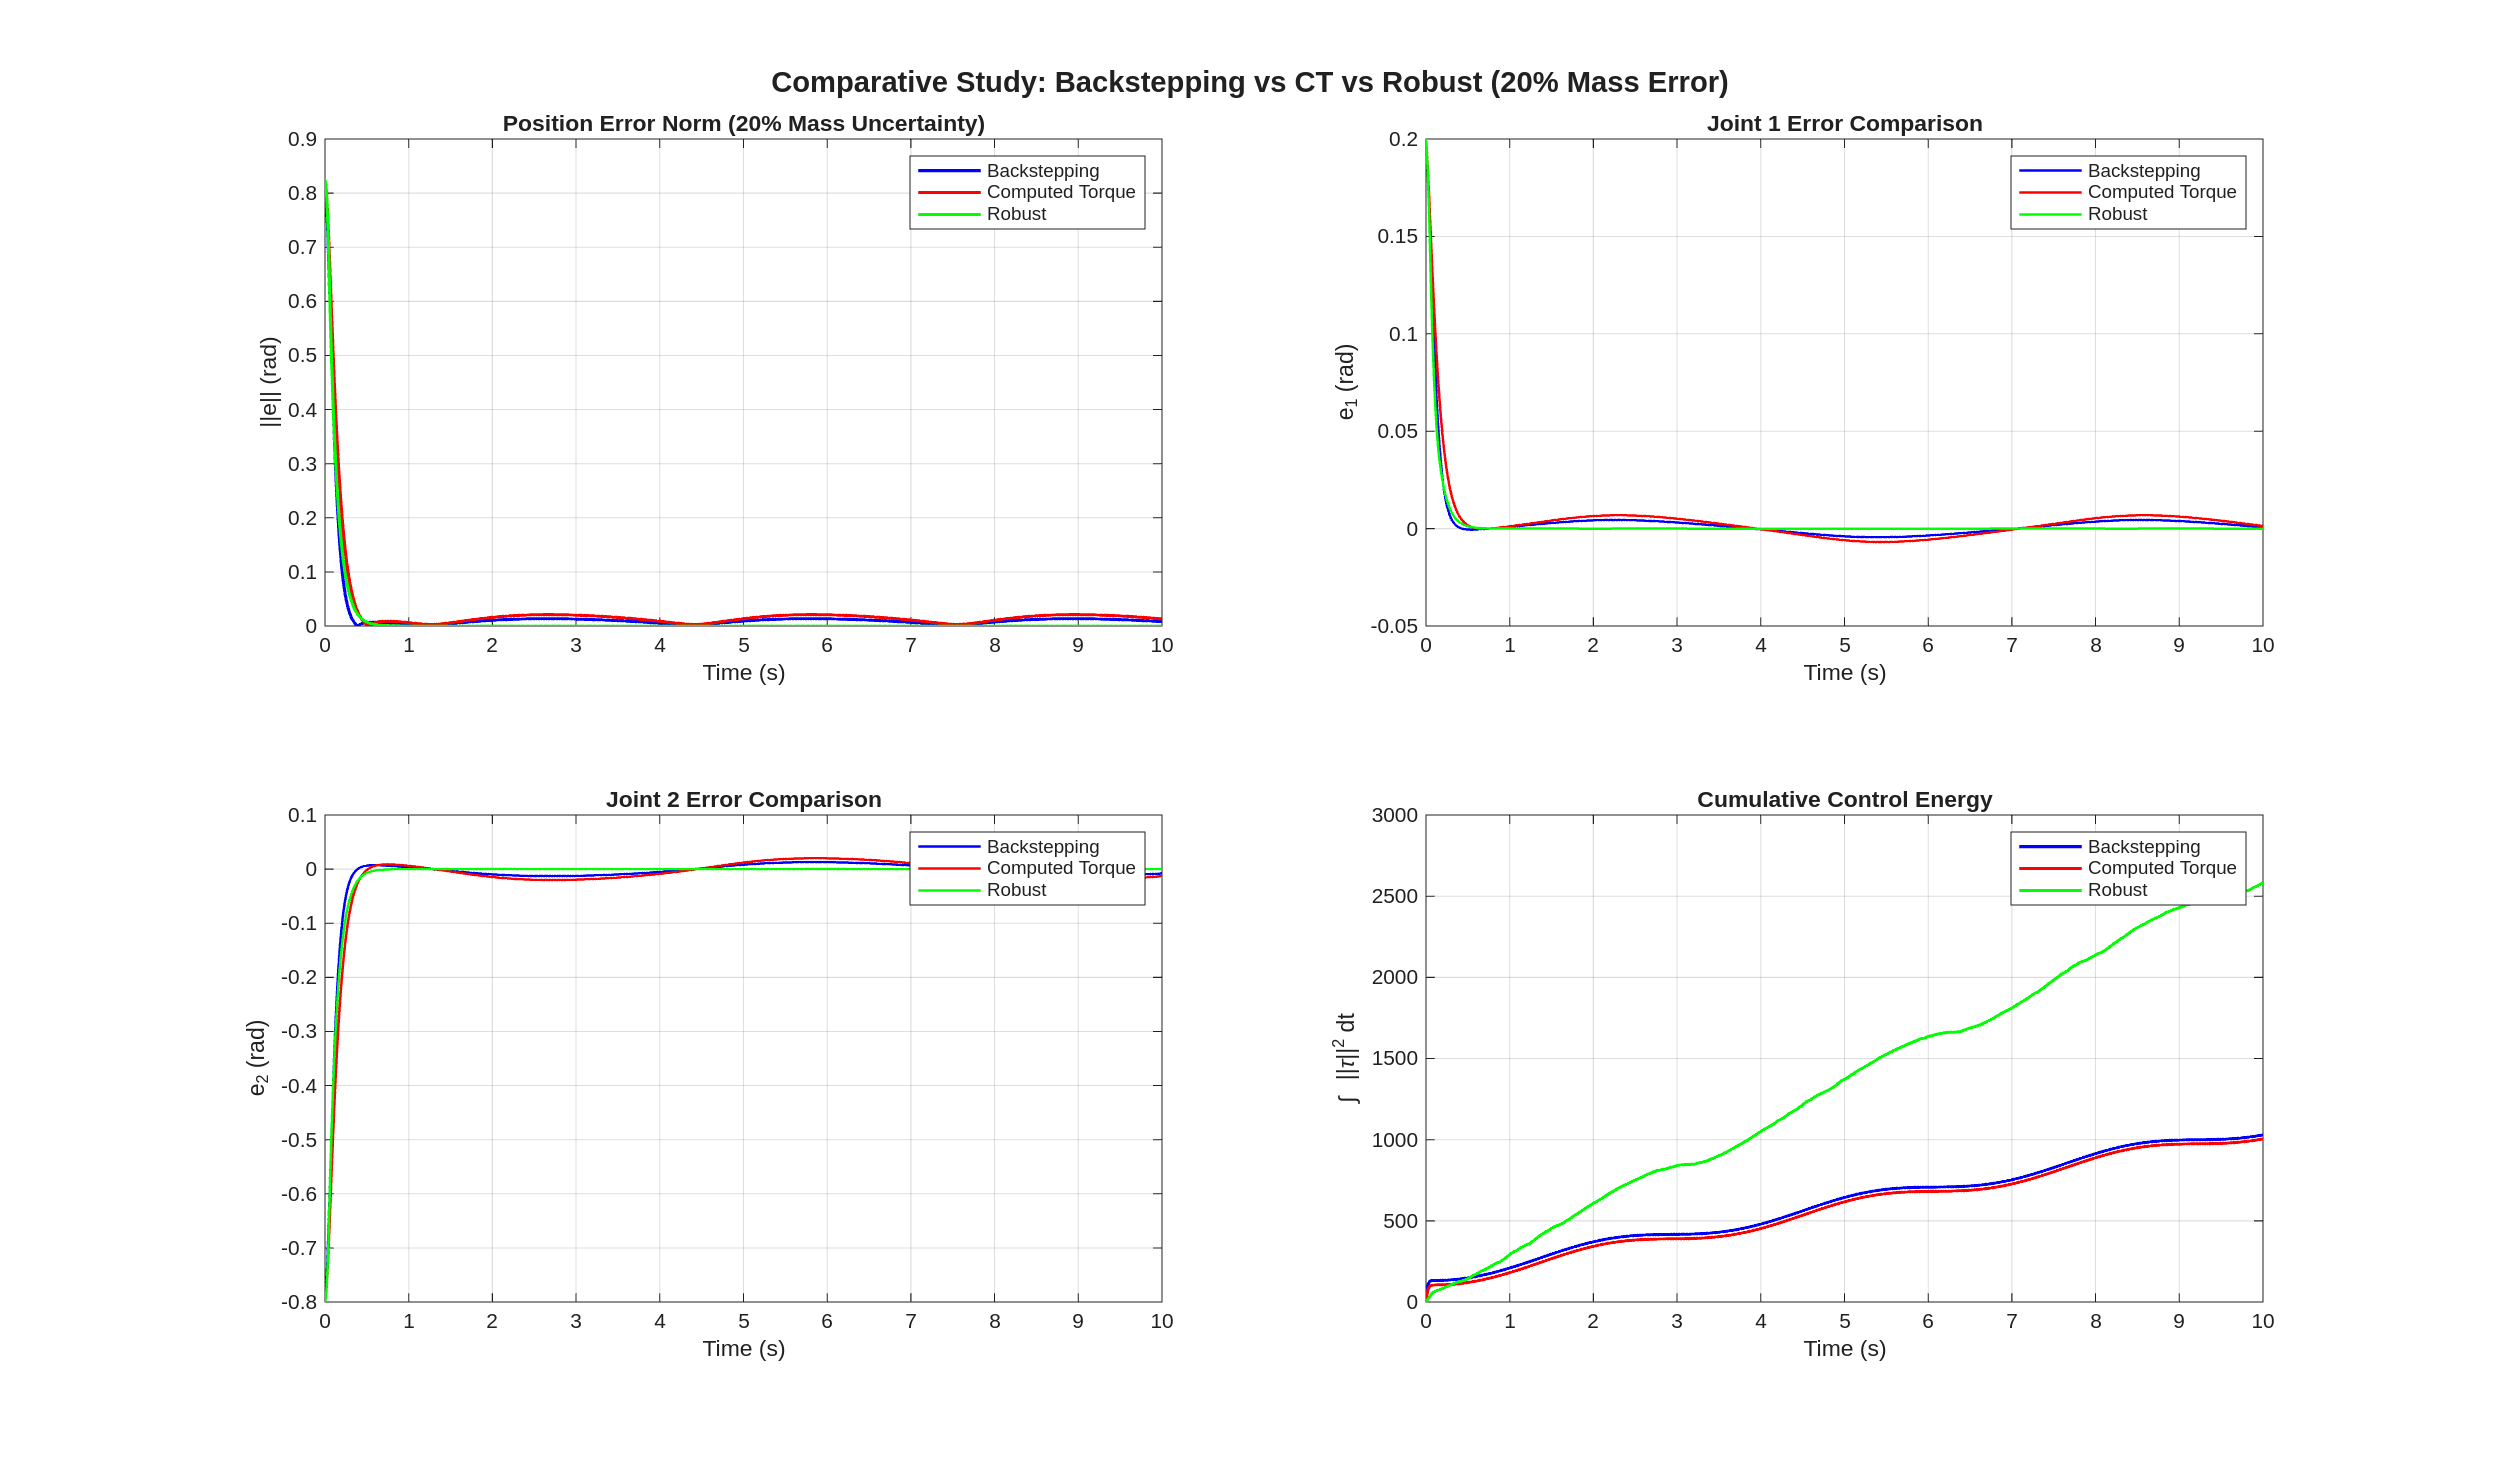
\includegraphics[width=0.92\textwidth,keepaspectratio]{images/week_07/Comparative_Study_With_Model_Uncertainty.png}
    \caption{Comparative study with model uncertainty.}
\end{figure}

\begin{figure}[ht]
    \centering
    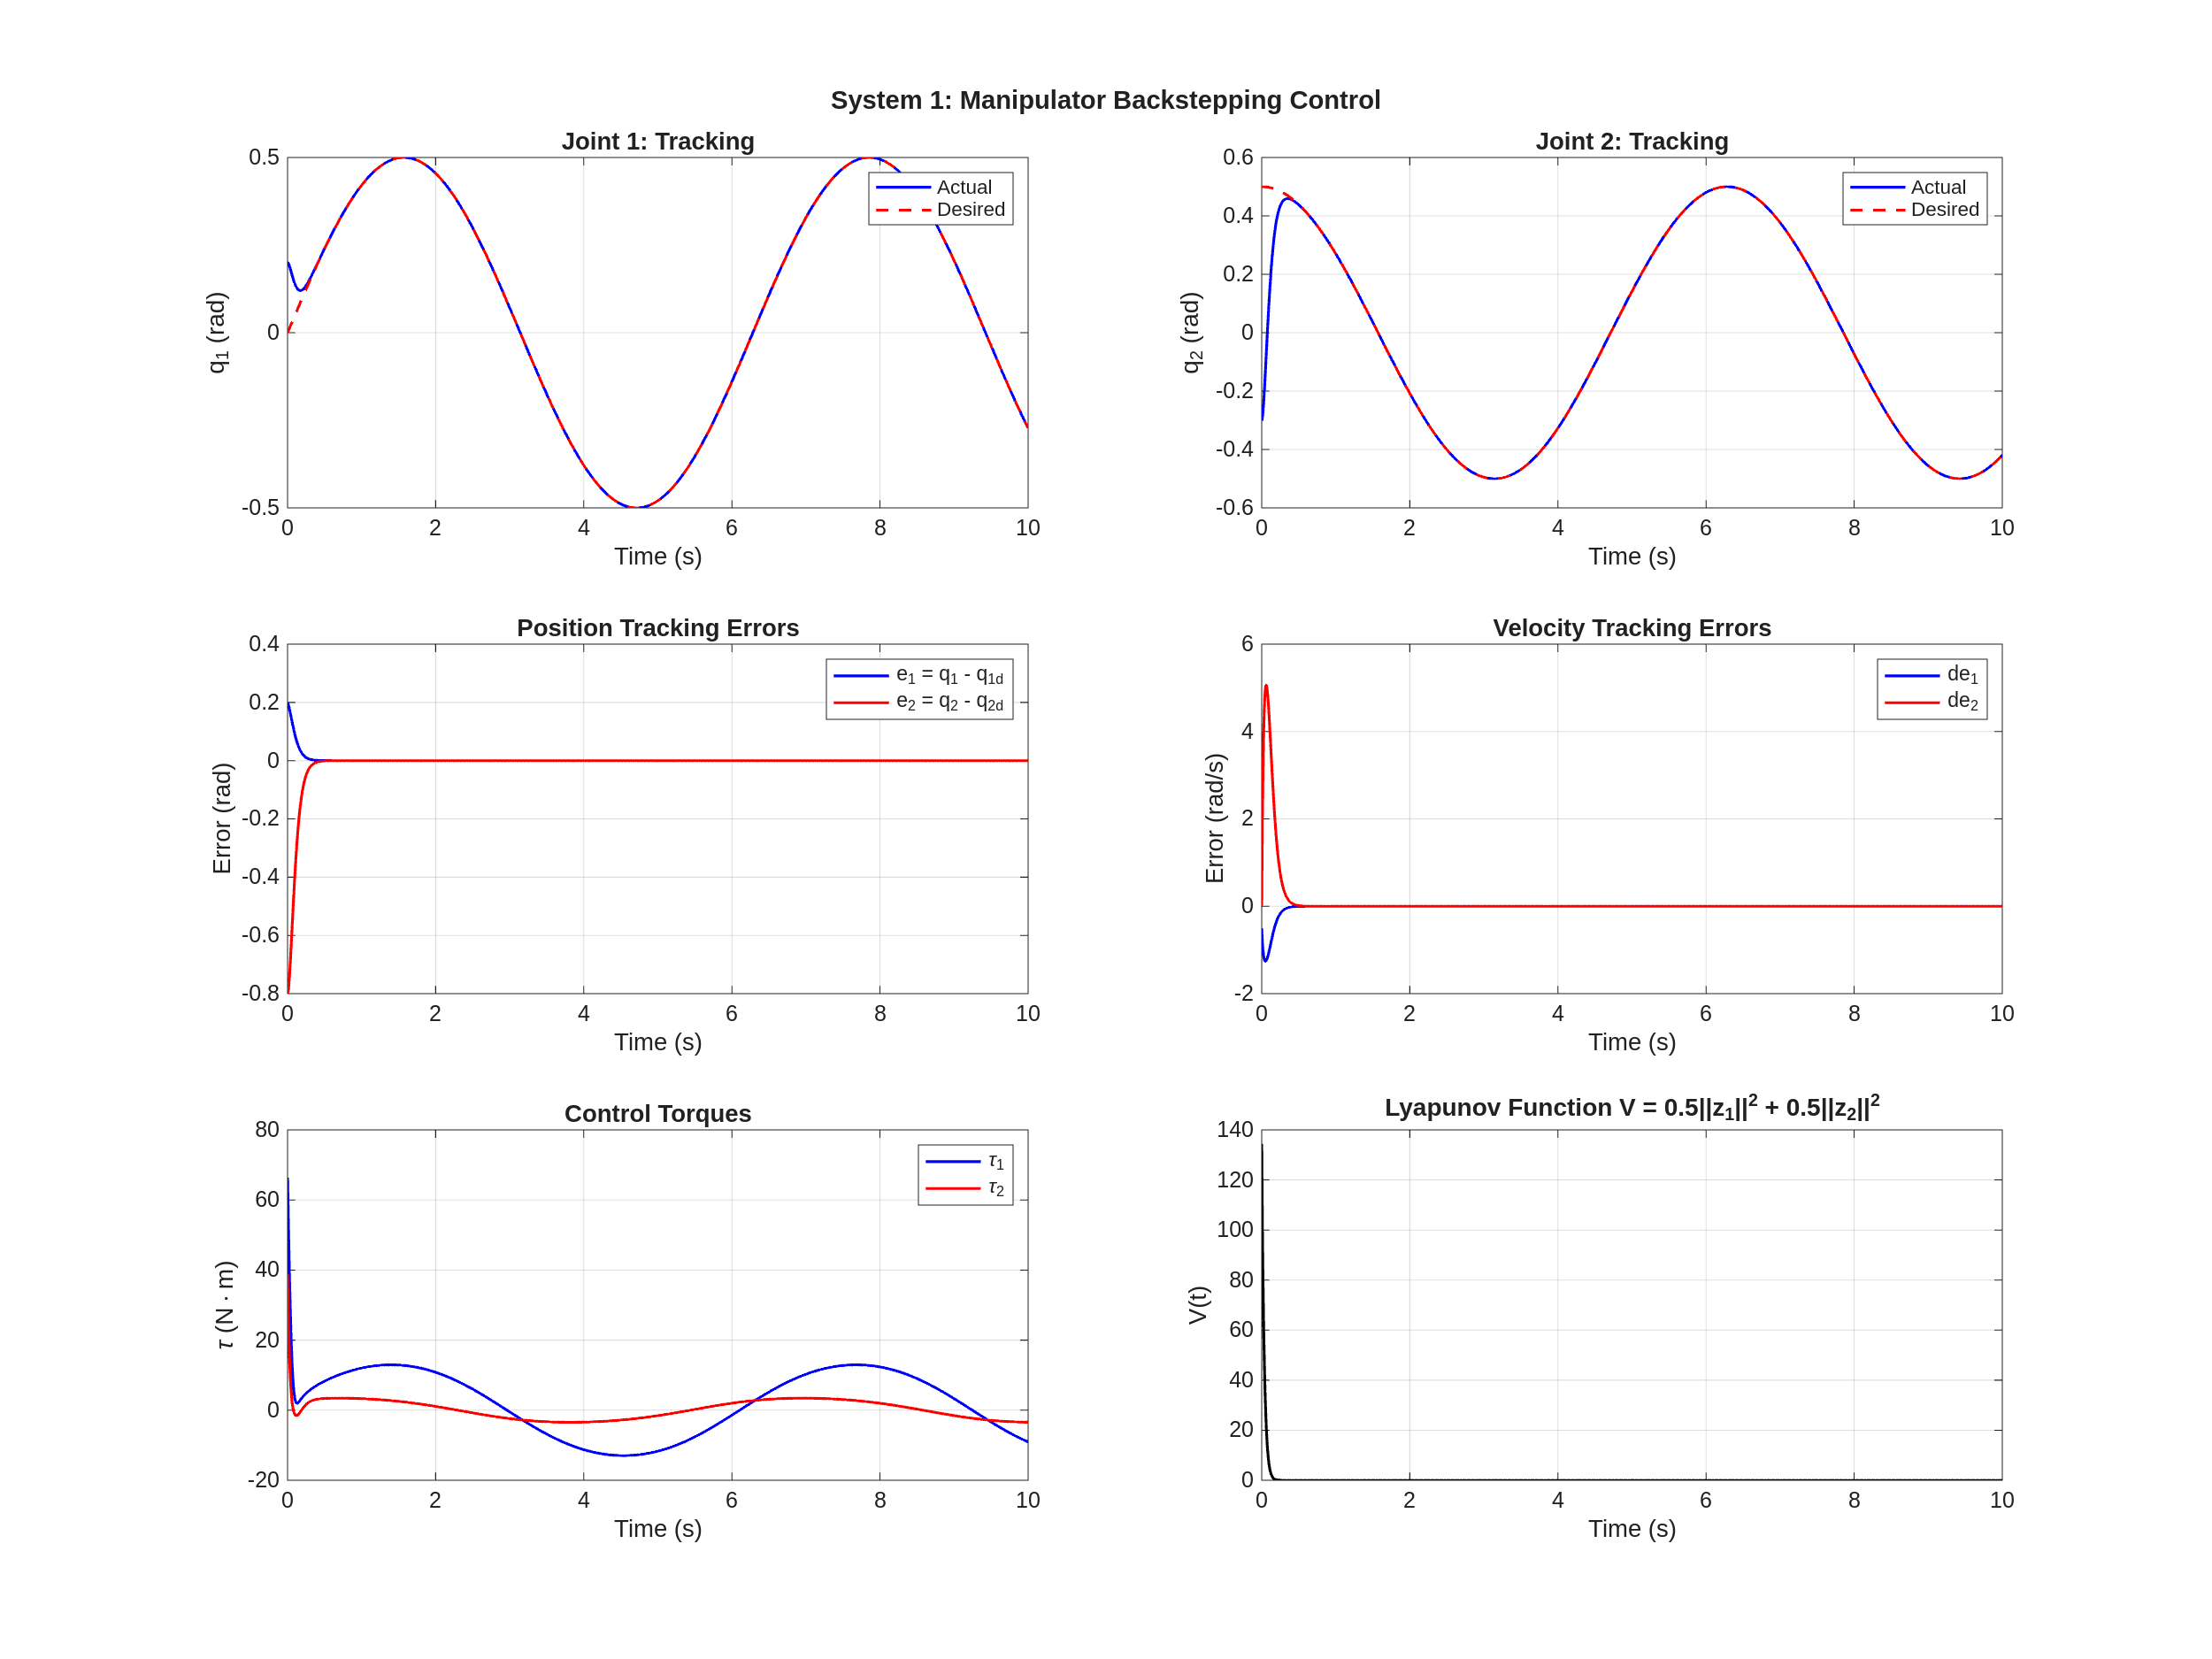
\includegraphics[width=0.92\textwidth,keepaspectratio]{images/week_07/Manipulator_Backstepping_Control.png}
    \caption{Manipulator backstepping control.}
\end{figure}

\begin{figure}[ht]
    \centering
    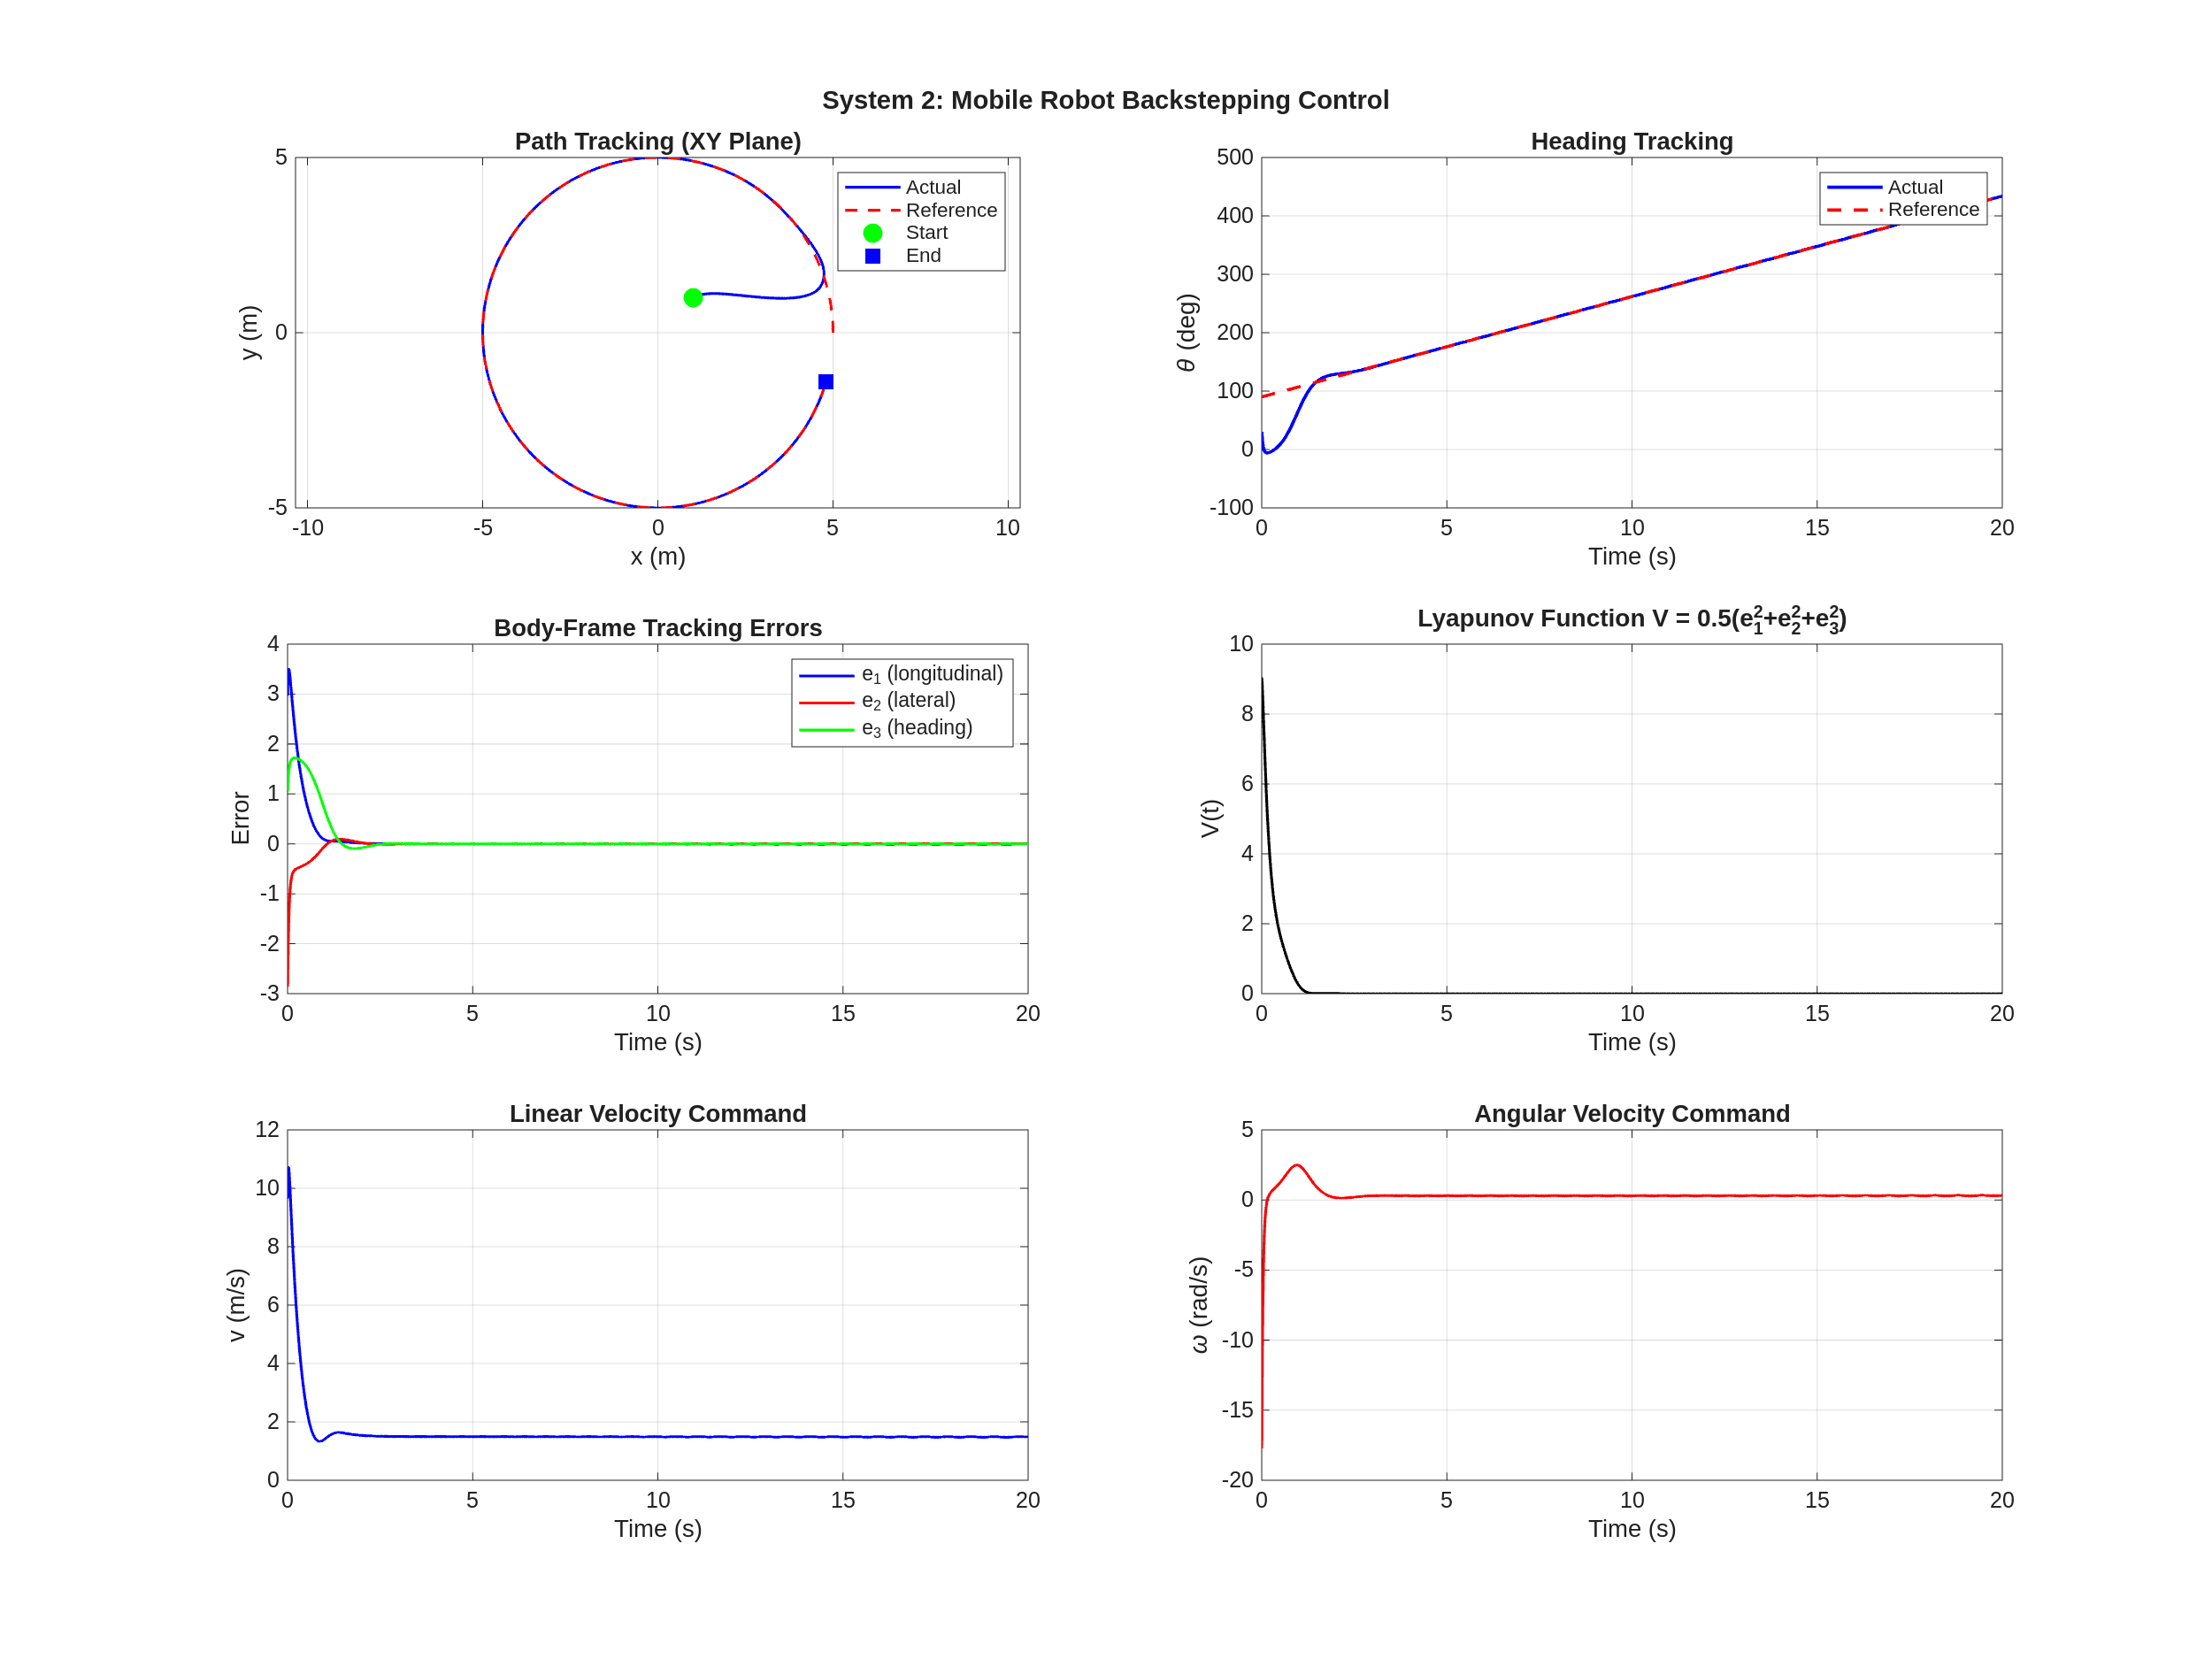
\includegraphics[width=0.92\textwidth,keepaspectratio]{images/week_07/Mobile_Robot_Backstepping_Control.png}
    \caption{Mobile robot backstepping control.}
\end{figure}

\begin{figure}[ht]
    \centering
    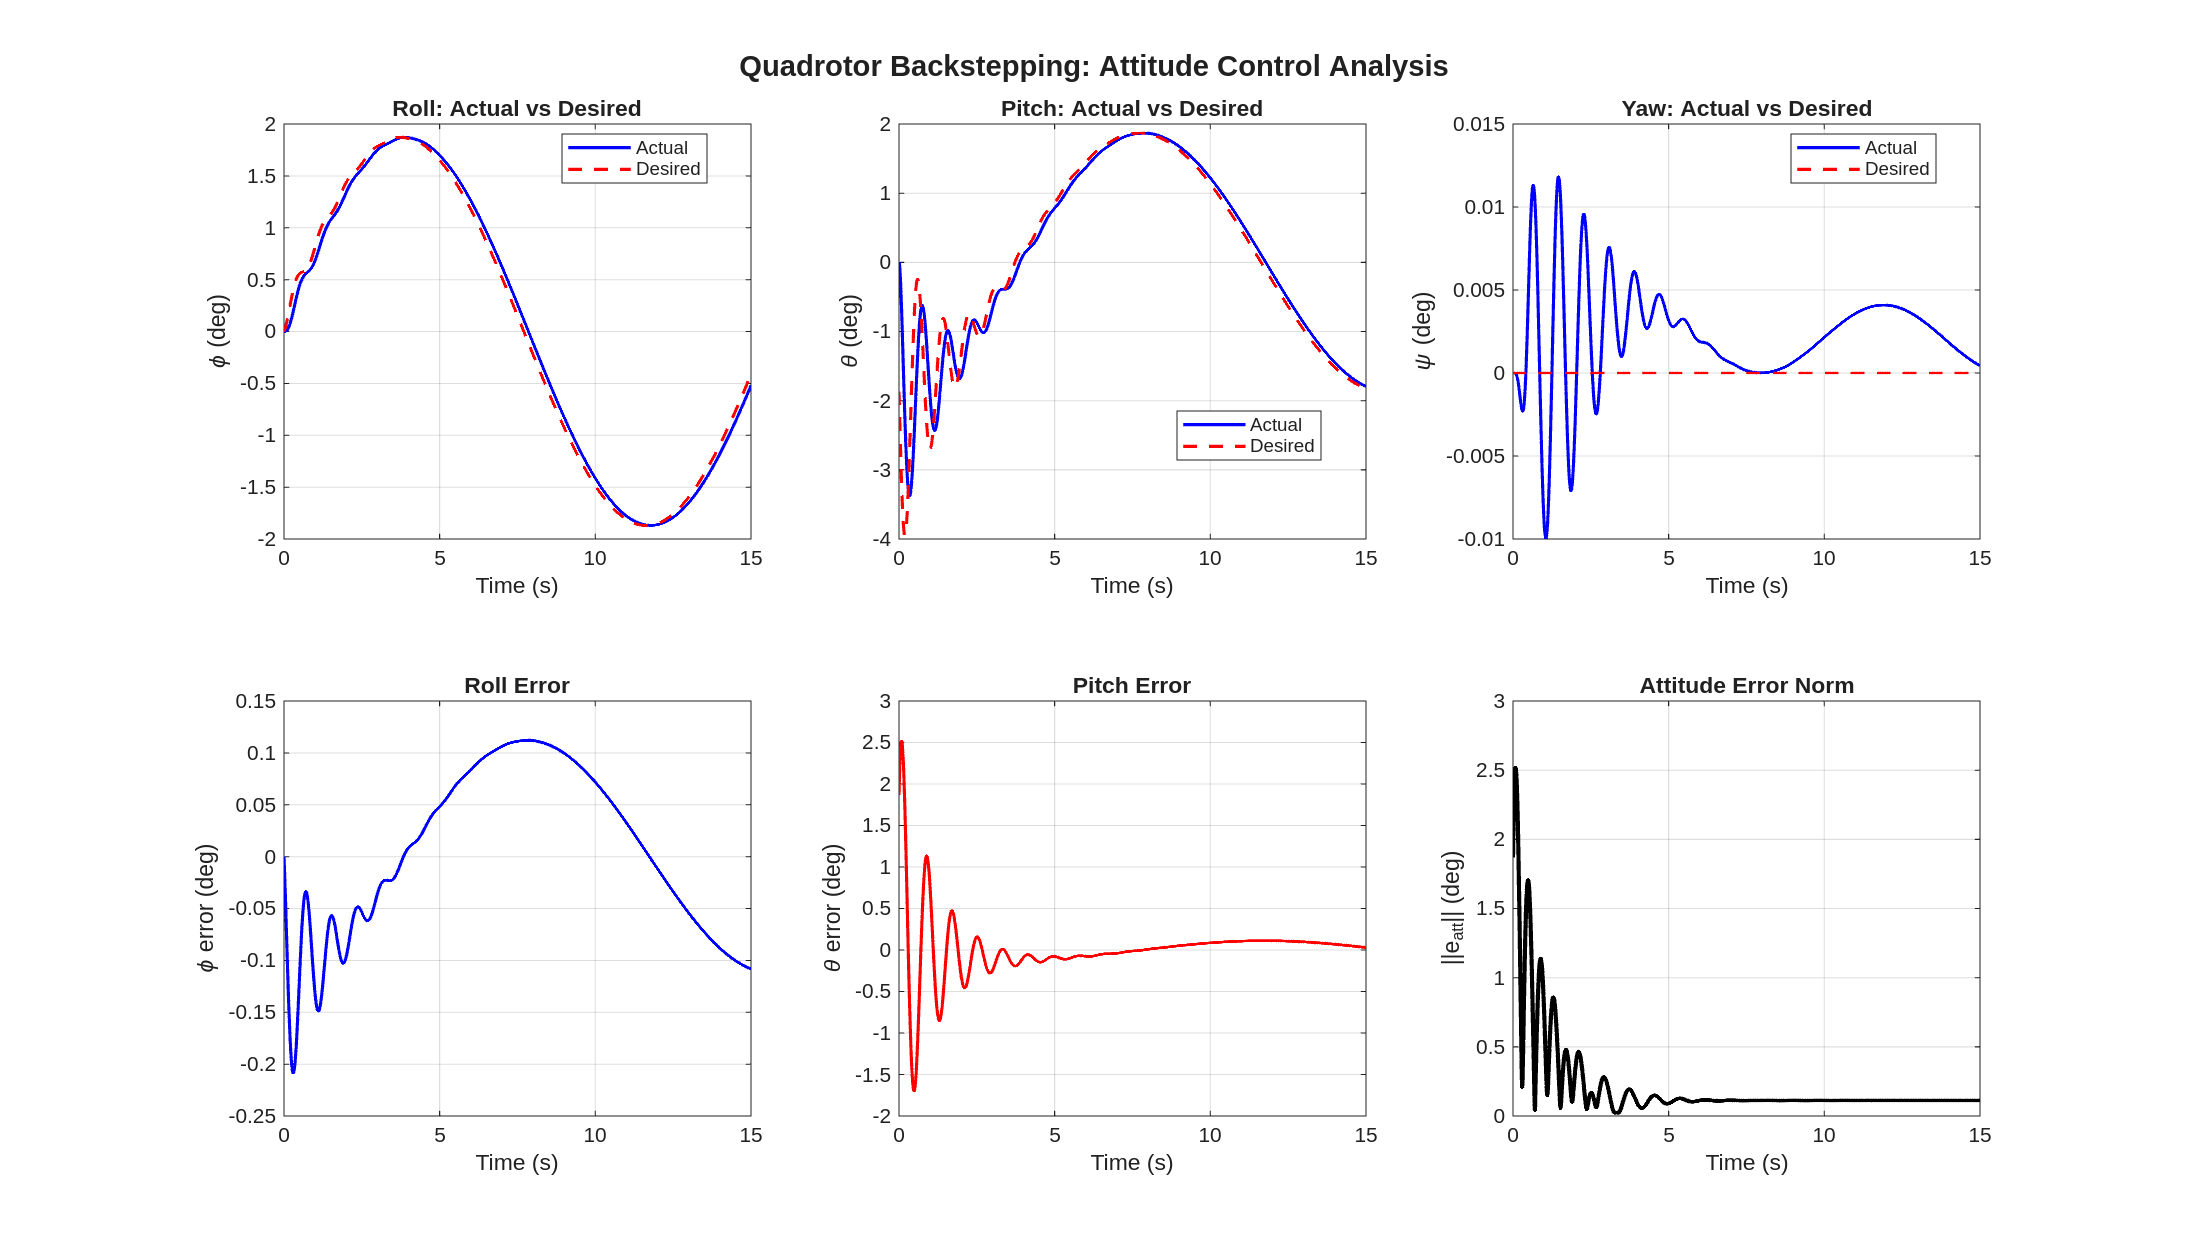
\includegraphics[width=0.92\textwidth,keepaspectratio]{images/week_07/Quad_Attitude_Control.png}
    \caption{Quad attitude control.}
\end{figure}

\begin{figure}[ht]
    \centering
    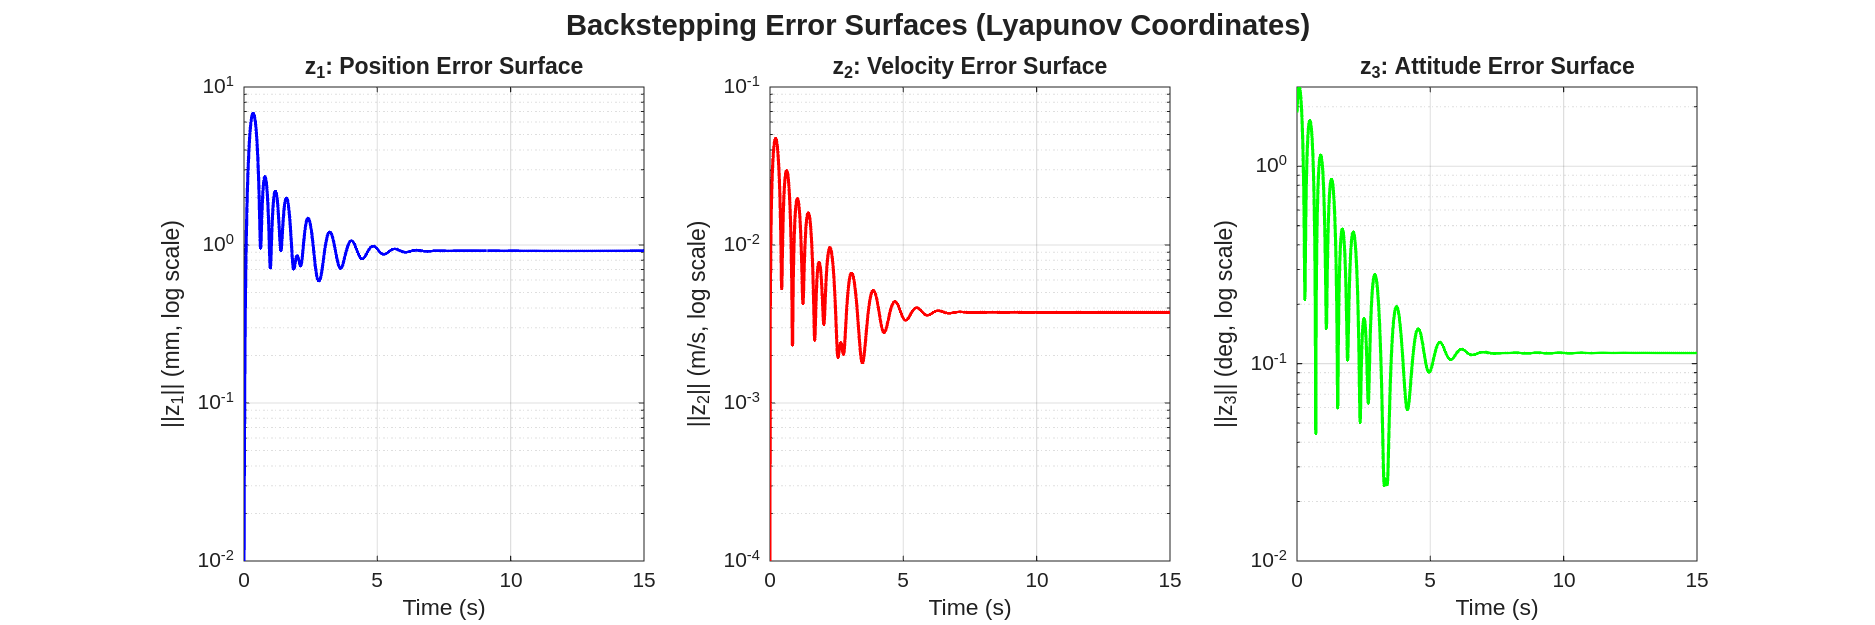
\includegraphics[width=0.92\textwidth,keepaspectratio]{images/week_07/Quad_Backstepping_Errors.png}
    \caption{Quad backstepping errors.}
\end{figure}

\begin{figure}[ht]
    \centering
    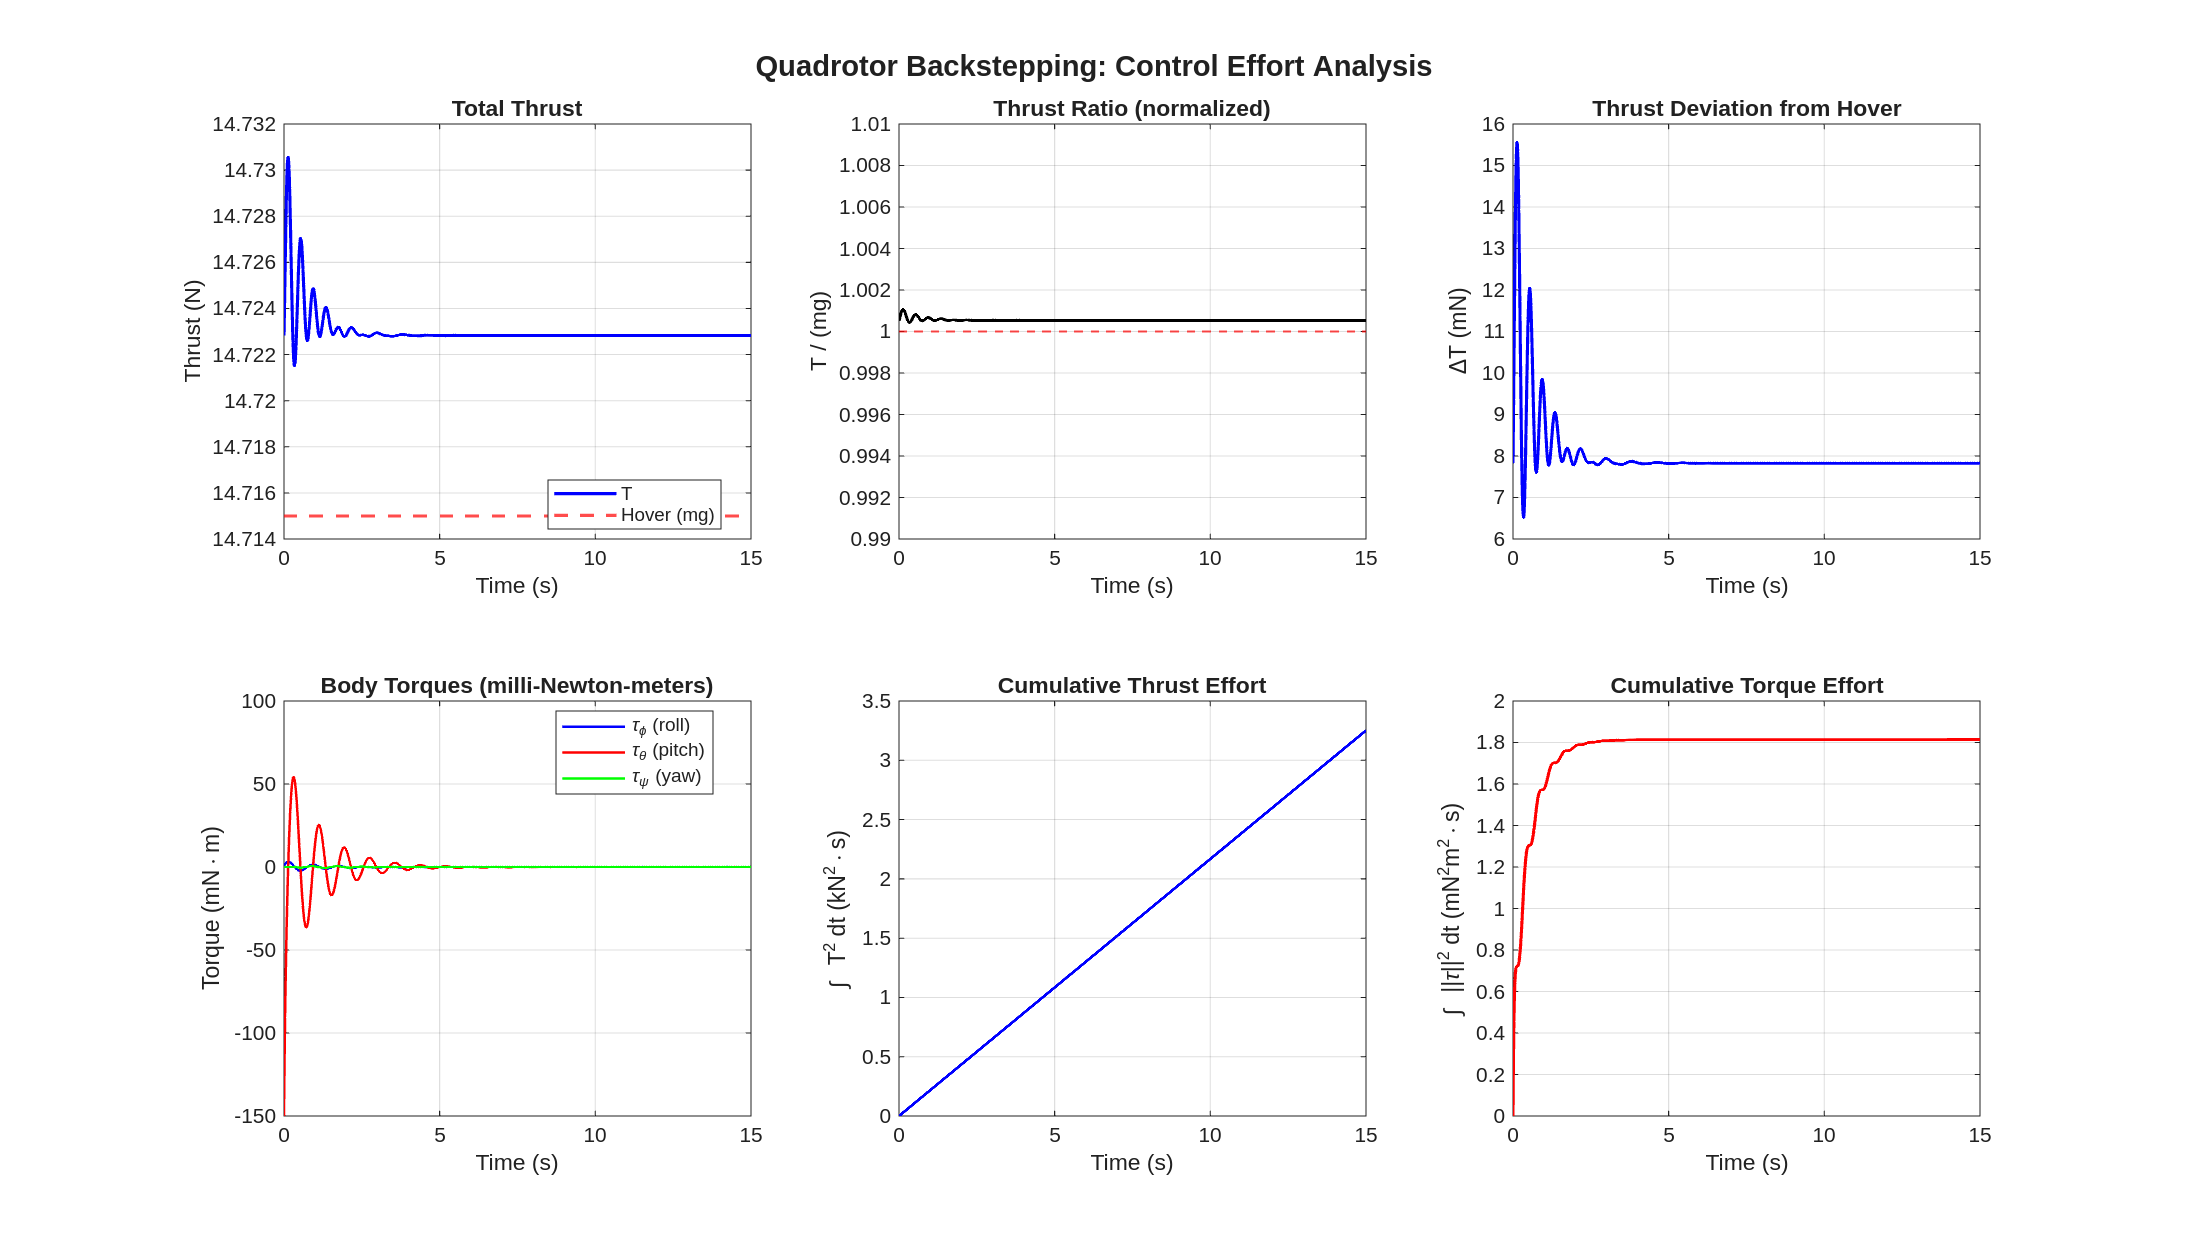
\includegraphics[width=0.92\textwidth,keepaspectratio]{images/week_07/Quad_Control_Effort.png}
    \caption{Quad control effort.}
\end{figure}

\begin{figure}[ht]
    \centering
    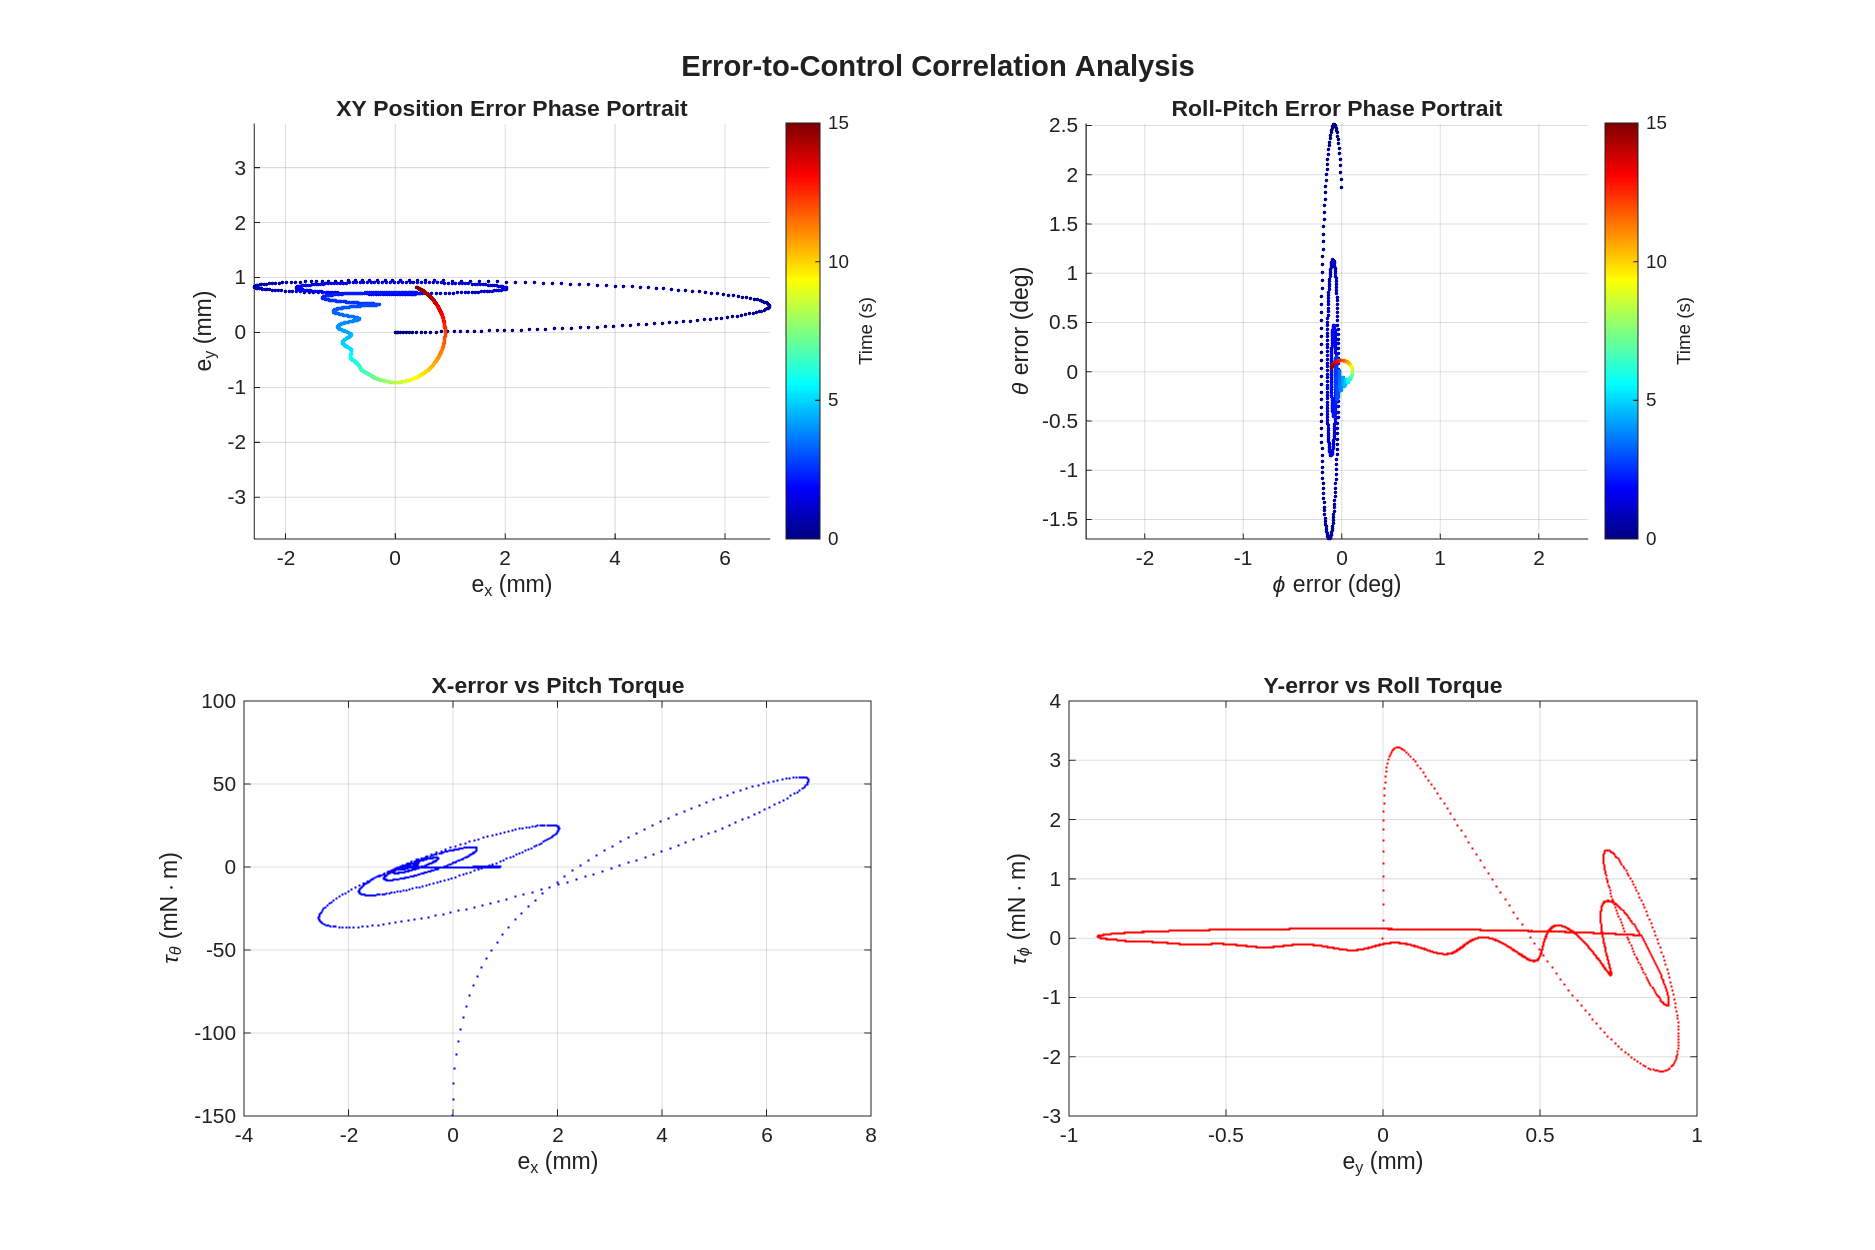
\includegraphics[width=0.92\textwidth,keepaspectratio]{images/week_07/Quad_Error_Control_Correlation.png}
    \caption{Quad error control correlation.}
\end{figure}

\begin{figure}[ht]
    \centering
    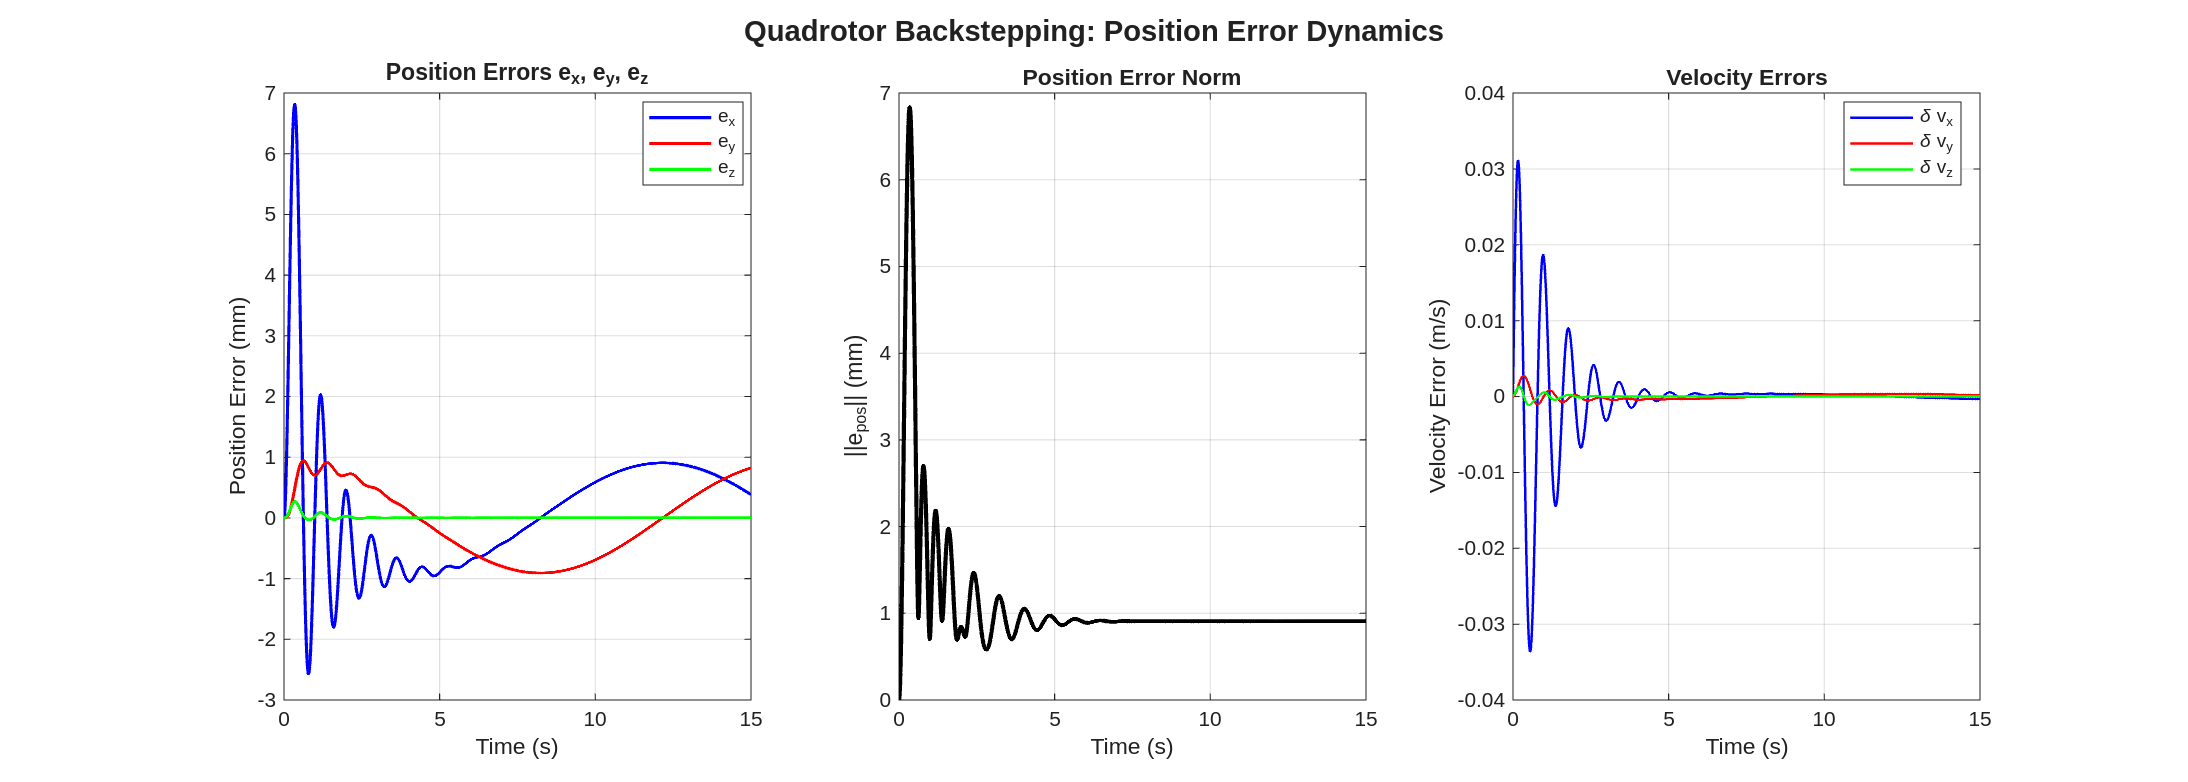
\includegraphics[width=0.92\textwidth,keepaspectratio]{images/week_07/Quad_Position_Error_Dynamics.png}
    \caption{Quad position error dynamics.}
\end{figure}

\begin{figure}[ht]
    \centering
    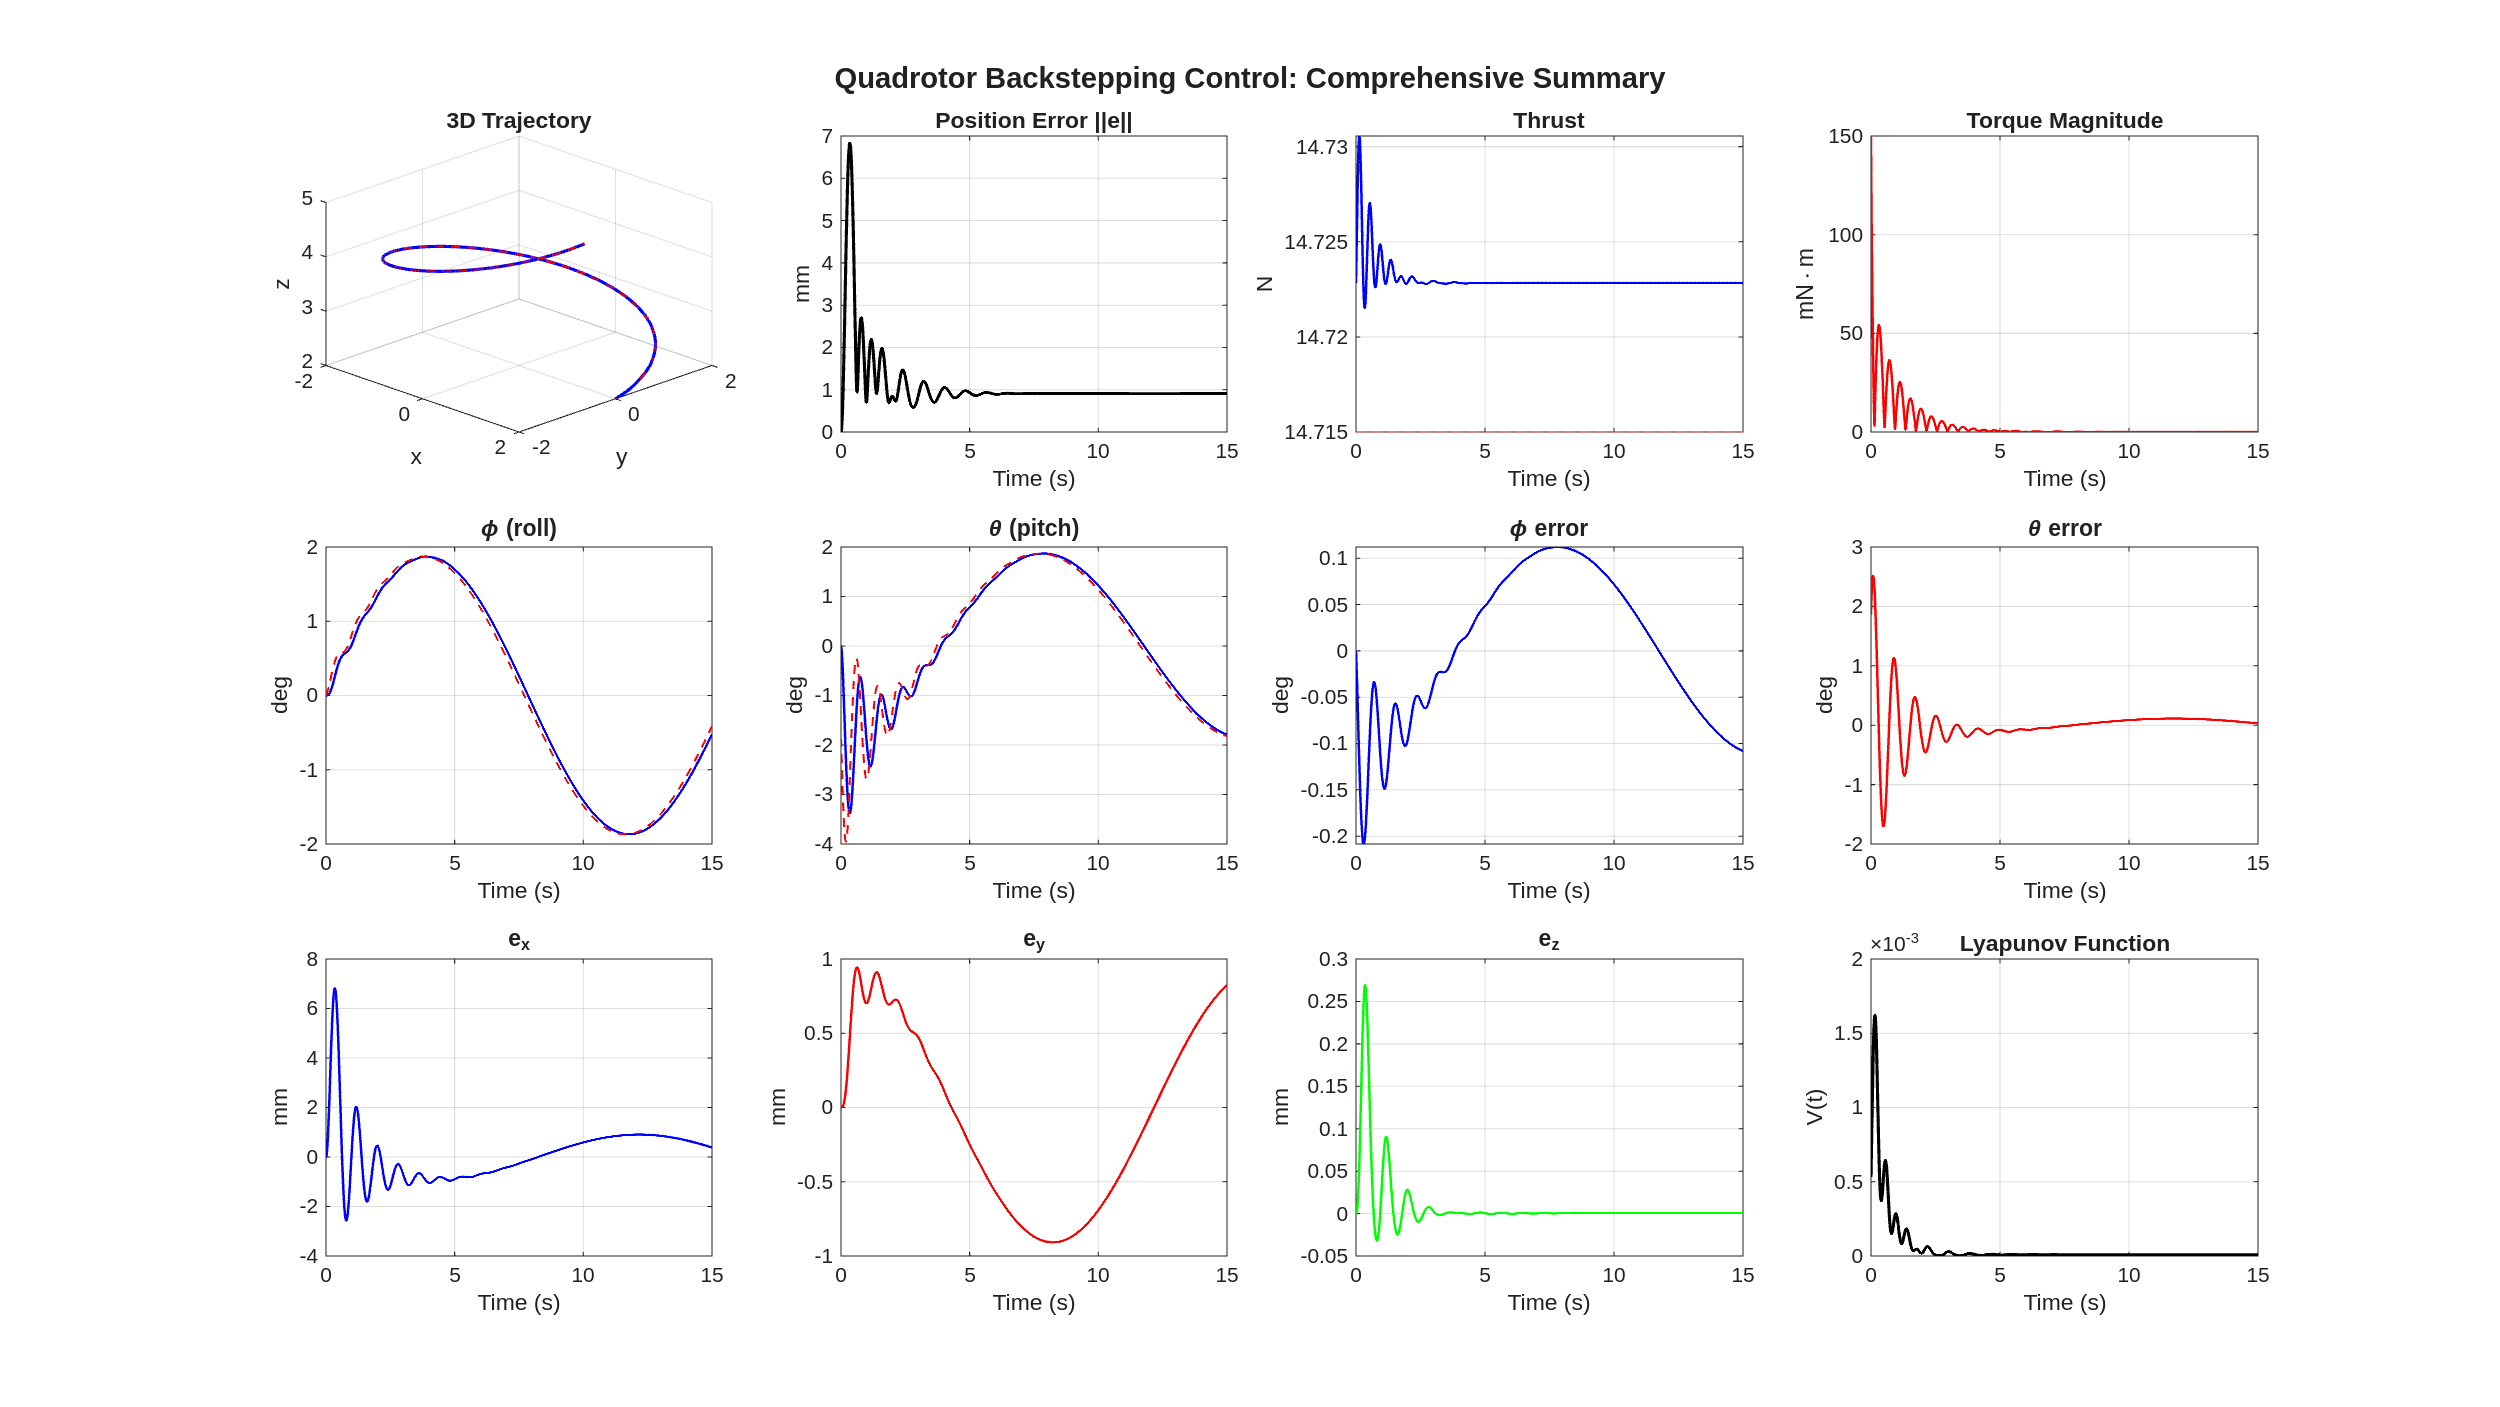
\includegraphics[width=0.92\textwidth,keepaspectratio]{images/week_07/Quad_Summary.png}
    \caption{Quad summary.}
\end{figure}

\begin{figure}[ht]
    \centering
    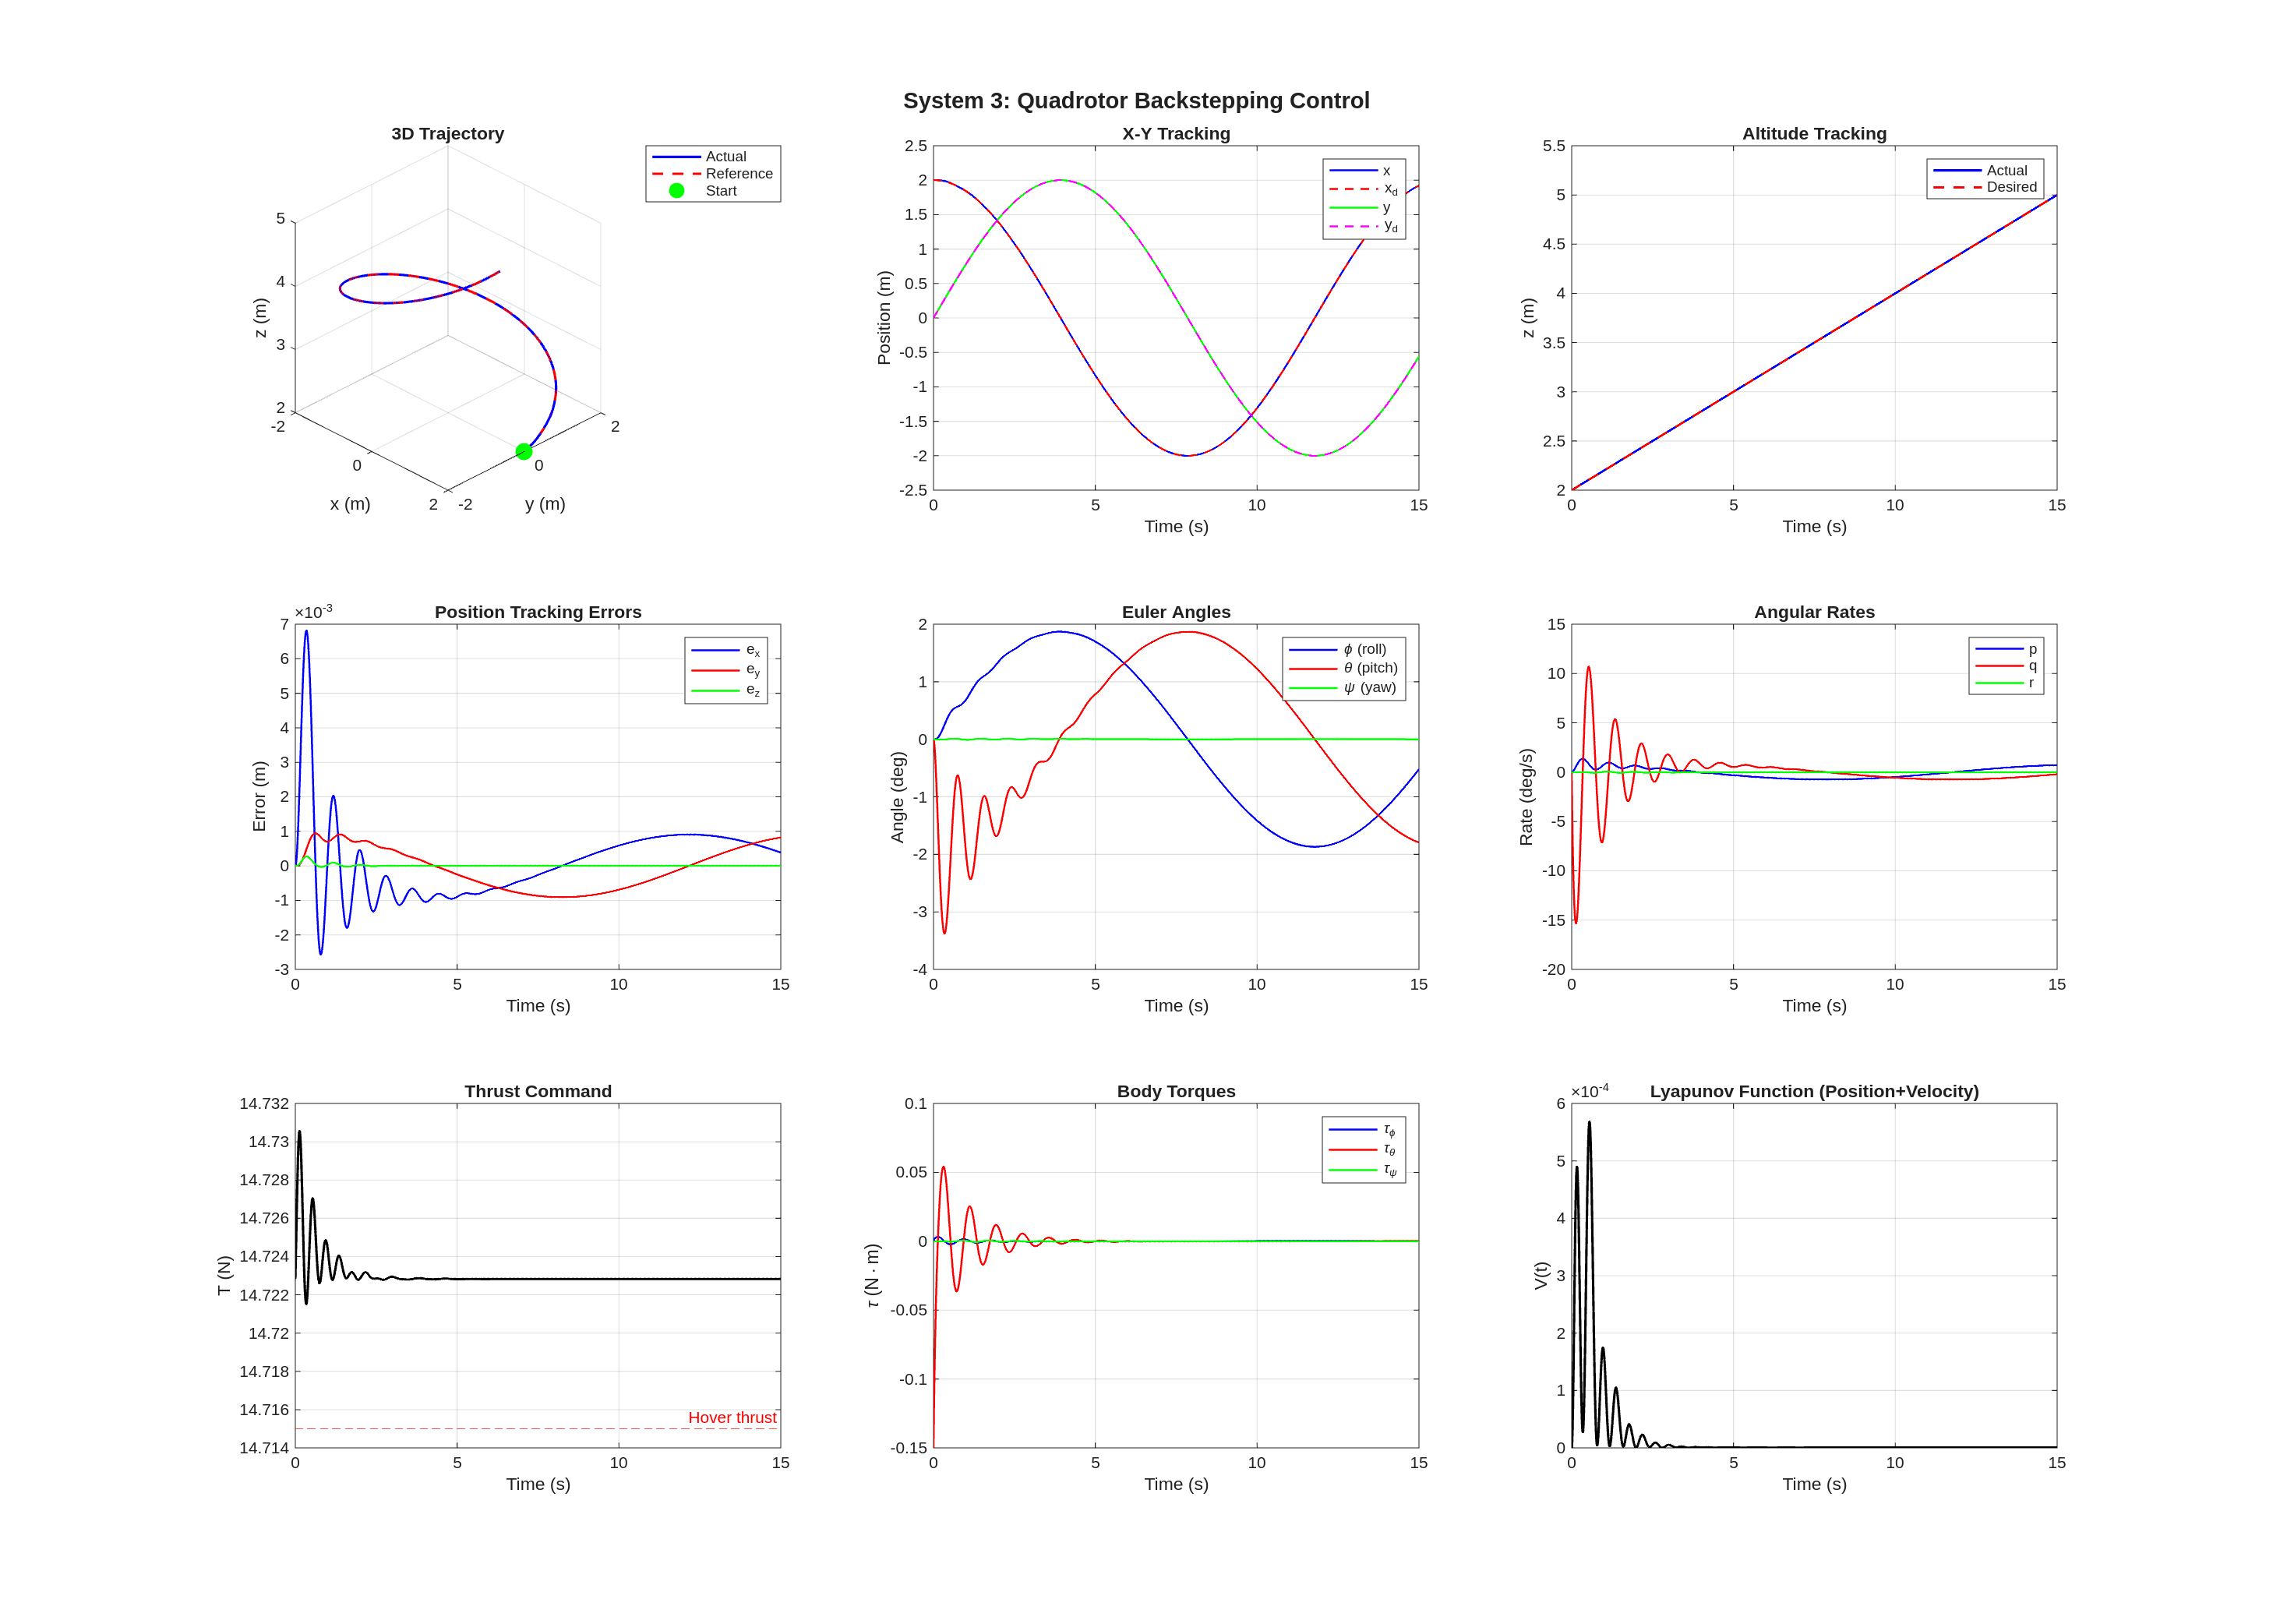
\includegraphics[width=0.92\textwidth,keepaspectratio]{images/week_07/Quadrotor_Backstepping_Control.png}
    \caption{Quadrotor backstepping control.}
\end{figure}

\section{Summary and Next Steps}

\subsection{Hands-on Activities \& Quiz}

\subsection{Activity 1: Gain Tuning for Manipulator Backstepping (10 min)}

Run \texttt{backstepping\_control\_simulation.m} and observe the manipulator plots.
Then modify the gains and re-run:

\begin{enumerate}
\tightlist
\item
  Set \(k_1 = 50, \; k_2 = 5\) (position gain much larger than velocity gain).
\item
  Set \(k_1 = 5, \; k_2 = 50\) (velocity gain much larger than position gain).
\item
  Set \(k_1 = k_2 = 25\) (balanced gains).
\end{enumerate}

\textbf{Expected observations:}

\begin{itemize}
\tightlist
\item
  \textbf{\(k_1 \gg k_2\):} Aggressive position correction generates large desired velocity changes.
  The velocity loop cannot track them fast enough, causing oscillatory or even unstable behaviour.
  The virtual control \(\alpha_1\) demands more than the torque loop can deliver.
\item
  \textbf{\(k_2 \gg k_1\):} The velocity error \(z_2\) converges quickly, but the position
  error \(z_1\) converges slowly because \(k_1\) is small. The system is overdamped
  with sluggish position tracking.
\item
  \textbf{\(k_1 \approx k_2\):} Balanced convergence rates for both loops. This is
  generally the best choice for smooth, fast tracking.
\end{itemize}

\subsection{Activity 2: Comparative Study (15 min)}

The MATLAB file includes a comparison of backstepping vs. computed torque vs. robust control
on the manipulator with model uncertainty (20\% mass error). Observe:

\begin{itemize}
\tightlist
\item
  Which controller has the smallest steady-state error?
\item
  Which controller has the smoothest control signal?
\item
  Which controller uses the least energy (smallest \(\int \|\tau\|^2 \, dt\))?
\end{itemize}

\subsubsection{Quiz --- Virtual Control Design}

\textbf{Q1:} Given the system \(\dot{x}_1 = x_1^2 + x_2\), \(\dot{x}_2 = x_2 + u\),
design a backstepping controller to stabilise \(x_1 = 0\).

\emph{Answer sketch:}

\begin{itemize}
\tightlist
\item
  Step 1: \(z_1 = x_1\), \(\dot{z}_1 = x_1^2 + x_2\).
  Choose \(\alpha_1 = -x_1^2 - k_1 x_1\) so that \(\dot{V}_1 = -k_1 x_1^2 + x_1 z_2\).
\item
  Step 2: \(z_2 = x_2 - \alpha_1\), \(\dot{z}_2 = x_2 + u - (2x_1)(x_1^2 + x_2) + k_1(x_1^2 + x_2)\).
  Choose \(u = -x_2 + \dot{\alpha}_1 - x_1 - k_2 z_2\).
\end{itemize}

\textbf{Q2:} In the two-step backstepping controller, what happens if we omit the
cross-coupling term \(-z_1\) from the torque law? Is stability still guaranteed?

\emph{Answer:} Without \(-z_1\), the Lyapunov derivative becomes
\(\dot{V}_2 = -k_1 z_1^2 - k_2 z_2^2 + z_1^T z_2\). The cross-term \(z_1^T z_2\) can be
positive, so \(\dot{V}_2\) is not guaranteed negative semi-definite. Stability is only ensured
if \(k_1 k_2 > \frac{1}{4}\) (by Young\textquotesingle s inequality), but the stability margin is reduced.
The systematic backstepping design avoids this issue entirely.

\textbf{Q3:} Why does the quadrotor need four backstepping steps while the
manipulator only needs two?

\emph{Answer:} The quadrotor has a four-level cascade:
position → velocity → orientation → angular rate, each acting as a virtual control
for the previous level. The manipulator only has two levels (position → velocity) because
the torque directly enters the velocity dynamics via \(M^{-1}\tau\). The number of backstepping
steps equals the relative degree from the output to the input.

\subsection{Summary: Comparison of All Five Control Methods}

\begin{table}[ht]\footnotesize\centering
\adjustbox{max width=\textwidth,max totalheight=0.85\textheight}{%
\begin{tabular}{llllll}

\topruleAspect & Computed Torque (Wk1) & MPC (Wk2) & Adaptive (Wk3) & Robust (Wk4) & Backstepping (Wk5) \\
\midrule\bottomrule\textbf{Core idea} & Cancel nonlinearity, impose linear error dynamics & Optimise predicted trajectory over finite horizon & On-line parameter estimation + control & Dominate worst-case bounded uncertainty & Recursive Lyapunov design through cascade structure \\
\textbf{Model requirement} & Exact model needed & Prediction model needed & Structure known, parameters unknown & Nominal model + uncertainty bound & Strict-feedback structure required \\
\textbf{Lyapunov function} & Implicit (linear closed-loop) & Cost function (not standard Lyapunov) & \(V = \frac{1}{2}s^T M s + \frac{1}{2}\tilde{\theta}^T\Gamma^{-1}\tilde{\theta}\) & \(V = \frac{1}{2}s^T M s\) & \(V = \sum \frac{1}{2}z_i^T W_i z_i\) (constructed step-by-step) \\
\textbf{Handles constraints} & No & Yes (core feature) & No (standard form) & No & No (standard form) \\
\textbf{Robustness} & Poor (sensitive to model errors) & Moderate (depends on model accuracy) & Good (adapts to parametric uncertainty) & Excellent (designed for uncertainty) & Good (Lyapunov-guaranteed; can add adaptation) \\
\textbf{Computation} & Low (closed-form) & High (on-line optimisation) & Moderate (adaptation law update) & Low (closed-form) & Moderate (derivatives of virtual controls) \\
\textbf{Key advantage} & Simple, well-understood & Handles constraints and preview & Self-tuning for unknown parameters & Guaranteed performance under uncertainty & Systematic design with constructive stability proof \\
\textbf{Key limitation} & No robustness to model error & Computational cost, model dependence & Needs persistent excitation, structured uncertainty & Conservative (worst-case design), chattering & Complexity explosion in \(\dot{\alpha}_i\) for high-order systems \\
\textbf{Control law form} & \(\tau = M(q)[\ddot{q}_d + K_D\dot{e} + K_P e] + C\dot{q} + G\) & \(u^* = \arg\min_{u} \sum_{k} \|x_k - x_r\|^2_Q + \|u_k\|^2_R\) & \(\tau = Y(q,\dot{q},\dot{q}_r,\ddot{q}_r)\hat{\theta} - K_D s\) & \(\tau = \hat{M}\ddot{q}_r + \hat{C}\dot{q}_r + \hat{G} - K_D s + \rho\frac{s}{\|s\|}\) & \(\tau = M[\ddot{q}_d - K_1\dot{z}_1 - K_2 z_2] + C\alpha_1 + G - z_1\) \\
\end{tabular}}
\end{table}


\textbf{Figure 8:} Side-by-side comparison of feedback linearization (cancels all nonlinearities) versus backstepping (exploits useful nonlinearities with constructive Lyapunov guarantees).

\textbf{Key takeaway:} Backstepping provides a \emph{systematic, constructive} methodology
for designing stabilising controllers for nonlinear systems in strict-feedback form.
Unlike computed torque, it does not blindly cancel all nonlinearities.
Unlike robust control, it does not require conservative worst-case bounds.
Its main challenge --- the "explosion of terms" as \(\dot{\alpha}_i\) grows with each step
--- can be addressed using \textbf{dynamic surface control} (a first-order filter on
each virtual control), which we may explore in future weeks.

\textbf{M.Sc. Control for Robots} --- AY 2025--26

Week 5: Backstepping Control --- Lecture Notes

These notes are for educational purposes.
Students are encouraged to verify all derivations independently.
